\section{Free fields, Ward identities and rotations}\label{sec:partII-G}

The only rotations that preserve the lattice, the Wilson action and the block-spin transformation of Sections~\ref{sec:partII-B}--\ref{sec:partII-F} are those of the hypercubic group~$\hypercubic$. Continuous rotational covariance of the limit is therefore an output of the construction. This section obtains it from a conserved stress tensor and proves Proposition~\ref{prop:MC}, Theorem~\ref{prop:ST} and Proposition~\ref{prop:SC}. The argument has three tasks.
\begin{enumerate}[label=(\arabic*)]
\item \emph{Find the conserved line.} The Maxwell comparison identifies the fields of degrees four and five with their free counterparts. A three-dimensional space of candidate tensors maps by divergence onto a two-dimensional space of vectors, so conserved tensors form a line (Lemma~\ref{lem:G2.2}).
\item \emph{Make the translation shell act as differentiation.} Shell fluxes of a member of that line define charge maps on the field spaces (Lemma~\ref{lem:G2.3}). Finite free Ward tests identify the translation charge with a multiple of differentiation (Lemma~\ref{lem:G3.1}).
\item \emph{Identify the angular action and recover rotations.} Coordinate reflection positivity controls the angular flux at infinity for collinear configurations, with no lower bound on the energy spectrum (Lemma~\ref{lem:G-collinear-flux}). Analyticity extends the angular identity to all configurations; finite internal tests remove the defect in the bracket relations, and the angular charges integrate to an $O(4)$ action (Lemma~\ref{lem:G3.1}).
\end{enumerate}
Section~\ref{sec:partII-G.1} treats the free field, Sections~\ref{sec:G-lattice}--\ref{sec:partII-G.2} the comparison and the conserved line, Section~\ref{sec:G-coordinate} the coordinate reflection spaces, and Section~\ref{sec:partII-G.3} the Ward identities. Section~\ref{sec:G-coordinate} uses no continuous rotation; continuous rotations are first available in Lemma~\ref{lem:G3.1}. The free calculation of Lemma~\ref{lem:G1.1} also supplies the positivity used in Lemma~\ref{lem:E2-free-tests}; its proof uses no interacting input.

Two estimates go beyond convergence at fixed separated points. The lattice comparison must control tests uniformly in their supremum norm, including near configurations with a shared coordinate; narrow strips around those configurations are removed, with different scales for the kernel and for its variation. Later, conservation removes the inner boundaries in the angular identity but not the boundary at infinity, which an anisotropic cutoff and the coordinate spectral estimates remove.

Except in the free calculation, fix the table, volume refinement, quotient fields and calculus of Definitions~\ref{def:D09}, \ref{def:D10} and~\ref{def:D11} and Lemmas~\ref{lem:F1}--\ref{lem:F3}. Subsequences below change only comparison radii. Write $\jmath_{d,e}$ for the inclusions and $\partial_a$ for field differentiation.

\subsection{Free fields}\label{sec:partII-G.1}

Put $z=x-y$ and $\mathsf h_{ab}(z)=\partial_a\partial_b\Gamma(z)$. The curvature covariance in Definition~\ref{def:D11} is
\begin{equation}\label{eq:G-curvature}
C_{ab,ij}(z)=-\delta_{bj}\mathsf h_{ai}+\delta_{bi}\mathsf h_{aj}
 +\delta_{aj}\mathsf h_{bi}-\delta_{ai}\mathsf h_{bj},\qquad
\mathsf h_{ab}=\frac{8z_az_b-2\delta_{ab}|z|^2}{4\pi^2|z|^6}.
\end{equation}
Different colours have zero covariance. Wick correlations sum products of covariances over the pairings that join factors of different insertions; for instance $\maxwellcorr_2({:}F_1F_2{:},{:}F_3F_4{:})=C_{13}C_{24}+C_{14}C_{23}$, and no covariance at zero separation enters. Set
\begin{equation}\label{eq:G-free-tensor}
\begin{aligned}
Q_{ab,ij}&=\sum_\alpha:F_{ab}^\alpha F_{ij}^\alpha:,
\qquad Q_{ab}=\sum_cQ_{ac,bc},\qquad Q_{\rm tot}=\sum_aQ_{aa},\\
\maxwellstress_{ab}&=-Q_{ab}+\tfrac14\delta_{ab}Q_{\rm tot},
\qquad \curvaturesquare=\tfrac14Q_{\rm tot}.
\end{aligned}
\end{equation}
The minus sign is fixed by the shell convention in Definition~\ref{def:D13}.

For the coordinate reflection $s_a$, strict reflected positivity of $u\in\maxwellspace{d}$ means
\begin{equation*}
\maxwellcorr_2(R^{\rm Max}(s_a)\bar u,u;s_ax,x)>0
\qquad(x=te_a,\ t>0).
\end{equation*}
Write $\mathsf L^{\rm Max}(K)$ for the derivative at zero of $R^{\rm Max}(e^{tK})$. The two free shell Ward identities, with the fluxes of Definition~\ref{def:D13}, are
\begin{equation}\label{eq:G-free-shells}
\mathcal P_b^{T^{\rm Max}}=S^{\rm Max}((\partial_b^{\rm Max}u)(x_0),\boldsymbol v(x)),\qquad
\mathcal Y_K^{T^{\rm Max}}=S^{\rm Max}((\mathsf L^{\rm Max}(K)u)(x_0),\boldsymbol v(x)).
\end{equation}

The next lemma gives the nondegeneracy of free correlation tests and the normalization used in the interacting comparison.
\begin{lemma}[Free positivity and stress]\label{lem:G1.1}
\begin{enumerate}[label=(\roman*)]
\item The Maxwell table satisfies E1--E7, the field calculus and $O(4)$ covariance.
\item Every $u\in\maxwellspace{d}\setminus\{0\}$ has strict reflected positivity.
\item The centered real symmetric $\hypercubic$-tensorial conserved degree-four tensors form the line $\R\maxwellstress$, and $\maxwellstress$ satisfies~\eqref{eq:G-free-shells}.
\item For $x\ne y$,
\begin{equation*}
\maxwellcorr_2(\curvaturesquare,\curvaturesquare;x,y)
=\frac{3\dimG}{\pi^4|x-y|^8}.
\end{equation*}
\end{enumerate}
\end{lemma}
\begin{proof}
\emph{(i)} Formula~\eqref{eq:G-curvature} satisfies Bianchi and $\sum_a\partial_a C_{ab,ij}=0$ off zero, so Wick correlations descend to the on-shell quotient. It also gives permutation symmetry, reality, units, translations and orthogonal covariance. Each differentiated contraction is homogeneous of a fixed negative degree and bounded on the unit sphere; a finite product of these bounds proves E6--E7. Differentiating the pairings proves the derivative law; inclusions retain the same polynomial. Reflection positivity E4--E5 is proved after~(ii).

\emph{(ii)} Kelvin inversion $z\mapsto z^\vee=z/|z|^2$ makes the reflected two-point pairing of curvature jets triangular with positive pivots~\eqref{eq:G-pivots}; strict positivity then follows from Wick's theorem. Let $\mathrm{Harm}_j$ be the real space of $\g$-valued homogeneous polynomial two-forms of degree~$j$ satisfying $df=\delta f=0$. Its Frobenius inner product identifies it with the dual of the order-$j$ on-shell curvature jets. Use Taylor coefficients $D^j/j!$ and the inner product summing both ordered form indices and ordered derivative indices; $p(\partial)$ denotes contraction with this normalized derivative. For $z\ne0$ put $\mathcal R_z=\mathbf 1_4-2zz^{\mathsf t}/|z|^2$. Let $R_p(y)$ be the covariance of $F(y)$ with the jet probe~$p$ at zero. Then
\begin{equation}\label{eq:G-kelvin}
R_p(y)=\varsigma_j|y|^{-4}(\mathcal R_y\otimes\mathcal R_y)p(y^\vee),
\qquad \varsigma_j=\frac{(j+1)(j+2)(-2)^j}{\pi^2}.
\end{equation}
Indeed $p(\partial)\Gamma=(-2)^j|y|^{-2j}p(y)\Gamma$; induction proves this, since traces of the coefficient tensor vanish by harmonicity. In the two curls, terms containing $\sum_a\partial_ap_{ab}$ and $\partial_ap_{bc}+\partial_bp_{ca}+\partial_cp_{ab}$ vanish. The remaining radial derivatives use $\sum_a y_a\partial_ap=jp$ and $\partial_a|y|^{-2j-2}=-(2j+2)y_a|y|^{-2j-4}$, and give $\varsigma_0=2/\pi^2$, $(j+1)\varsigma_{j+1}=-2(j+3)\varsigma_j$.

For towers $p=(p_j)$ and $q=(q_j)$, let $B_z(p,q)$ be their two-site covariance at separation~$z$, with $\mathcal R_z$ acting on all tensor indices of the second probe; this is the reflected jet pairing at $\pm z/2$. Define the triangular map~$\sigma_z$ by replacing a single order-$j$ probe~$p$ with the tower whose order-$k$ component is $(\varsigma_j/\varsigma_k)T_k[p(\cdot-z^\vee)]$, $k\le j$, where $T_k$ is the homogeneous Taylor term at zero. Its generated field is the right side of~\eqref{eq:G-kelvin} with $p(y^\vee-z^\vee)$. Since $D(z^\vee)=|z|^{-2}\mathcal R_z$, its Taylor terms at~$z$ below~$j$ vanish, and its top term is $\varsigma_j|z|^{-2j-4}\mathcal R_zp$. Symmetry removes the entries above the diagonal. Thus
\begin{equation}\label{eq:G-pivots}
B_z(\sigma_zp,\sigma_zq)
 =\sum_j\frac{(j+1)(j+2)2^j}{\pi^2|z|^{2j+4}}
 \langle p_j,q_j\rangle.
\end{equation}
Evaluating the second order-$j$ probe supplies $(-1)^j$, since its positional derivatives are opposite to derivatives of the separation; this cancels the sign in~$\varsigma_j$. In coordinates diagonalizing this form, Wick pairing between two sites gives $\langle X^\mu,X^\nu\rangle=\mathbf1_{\mu=\nu}\mu!\prod_i b_i^{\mu_i}$ with $b_i>0$. Every polynomial uses a finite tower, proving strict positivity.

For several positive-side sites the reflected curvature covariance is positive semidefinite: spatial Fourier transformation of~$\Gamma$ gives $e^{-|p|(t+s)}/(2|p|)$, and its two curls, with reflection of the form indices, give the sum of squares of the two transverse polarizations. Jet derivatives differentiate the same factors. Include the contractions within each positive-side word in its Fock vector; its reflected pairing is then the symmetric Fock pairing of this positive semidefinite form, so finite sums of words have nonnegative squared norm. On compact separated supports every pairing is continuous and bounded; integration gives E5 and point evaluation gives E4.

\emph{(iii)} Simplicity makes every invariant linear colour form zero and every invariant bilinear form a multiple of the fixed metric. Through weight four only the unit and the quadratics~$Q$ remain, and sign changes and permutations give the basis
\begin{equation*}
Z^{(1)}_{ab}=\delta_{ab}Q_{aa},\qquad
Z^{(2)}_{ab}=\delta_{ab}(Q_{\rm tot}-2Q_{aa}),\qquad
Z^{(3)}_{ab}=(1-\delta_{ab})Q_{ab}
\end{equation*}
of centered real symmetric tensors. Sign parity reduces their divergences to contractions of $F\partial F$ with the free index~$b$. The equations remove $\sum_d\partial_dF_{dc}$, and Bianchi gives $2\sum_{c,d}F_{cd}\partial_cF_{bd}=\sum_{c,d}F_{cd}\partial_bF_{cd}$. So the divergences lie in the plane spanned by
\begin{equation*}
\sum_c:F_{bc}\partial_bF_{bc}: =\tfrac12\partial_bQ_{bb},\qquad
\sum_{c<d,\ c,d\ne b}:F_{cd}\partial_bF_{cd}: =\tfrac14\partial_b(Q_{\rm tot}-2Q_{bb}),
\end{equation*}
with colour sums understood. Test the first components of the divergences of $Z^{(1)},Z^{(2)},Z^{(3)}$ (columns) at~$e_1$ against $Q_{12,12}(0)$ and $Q_{23,23}(0)$ (rows), dividing by $\dimG/(4\pi^2)^2$. For example $S^{\rm Max}_2(Q_{11}(te_1),Q_{12,12}(0))=2\dimG/(\pi^4t^8)$, whose derivative gives the first entry; differentiating~\eqref{eq:G-curvature} gives the others:
\begin{equation}\label{eq:G-divergence-matrix}
\begin{pmatrix}-256&0&128\\0&-512&-128\end{pmatrix}.
\end{equation}
Its first two columns are independent, so divergence maps the span of the $Z^{(i)}$ onto this plane. The test of $Z^{(3)}_{12}$ against $Q_{13,23}$ gives $-16$, and zero for $Z^{(1)},Z^{(2)}$, so the three tensors are independent. The kernel is the line of $\tfrac12Z^{(1)}-\tfrac14Z^{(2)}+Z^{(3)}=-\maxwellstress$.

To compute its charge, polarize~$\maxwellstress$ between a smooth Maxwell wave~$f$ and the field~$g$ generated by a probe at~$x_0$. Replace $\Gamma$ by $\Gamma_\varepsilon$ with $-\Delta\Gamma_\varepsilon=\rho_\varepsilon$, a smooth approximate identity. For a probe $F_{ij}$ the divergence of~$g$ is $\delta_{bj}\partial_i\rho_\varepsilon-\delta_{bi}\partial_j\rho_\varepsilon$. The polarized tensor is $t_{ab}=-\sum_c(f_{ac}g_{bc}+g_{ac}f_{bc})+\tfrac12\delta_{ab}\sum_{i,j}f_{ij}g_{ij}$, and Bianchi gives $\sum_a\partial_at_{ab}=-\sum_c f_{bc}\sum_a\partial_ag_{ac}$. With the minus sign of the shell integral, $\int\chi v_b\partial_at_{ab}=-\int\chi v_b f_{bc}(\delta_{cj}\partial_i\rho_\varepsilon-\delta_{ci}\partial_j\rho_\varepsilon)$, and a second integration by parts gives
\begin{equation*}
\partial_i(v_bf_{bj})(x_0)-\partial_j(v_bf_{bi})(x_0)
 =(\mathrm{Lie}_vf)_{ij}(x_0).
\end{equation*}
No derivative of~$\chi$ appears at~$x_0$, and the contraction with~$Dv$ vanishes by symmetry. For $v=K(\cdot-x_0)$ this is $\sum_c(K_{ci}f_{cj}+K_{cj}f_{ic})(x_0)$, the generator of the free action on curvature; for constant~$v$ it is $v\cdot\nabla f$. Higher probes follow by differentiating in~$x_0$. In a Wick contraction, the terms in which both stress legs end at~$x_0$ contribute zero to the shell flux: dilation by~$2$ multiplies their shell integral by $2^{3+p-8-j-l}\ne1$ (probe orders~$j,l$, weight degree $p=0,1$), while the flux is independent of the cutoff. Terms with both legs outside vanish by conservation. The remaining contractions give the derivation~$\mathrm{Lie}_v$, proving~\eqref{eq:G-free-shells}.

\emph{(iv)} At~$z=re_1$ the six unordered curvature components have diagonal covariances $\pm(\pi^2r^4)^{-1}$. Since $\curvaturesquare=\tfrac12\sum_{a<b,\alpha}{:}(F_{ab}^\alpha)^2{:}$, its two-point Wick sum is $\tfrac14\cdot2\cdot6\dimG/(\pi^4r^8)$. Orthogonal covariance gives the formula for every~$z\ne0$.
\end{proof}

\begin{figure}[t]
\centering
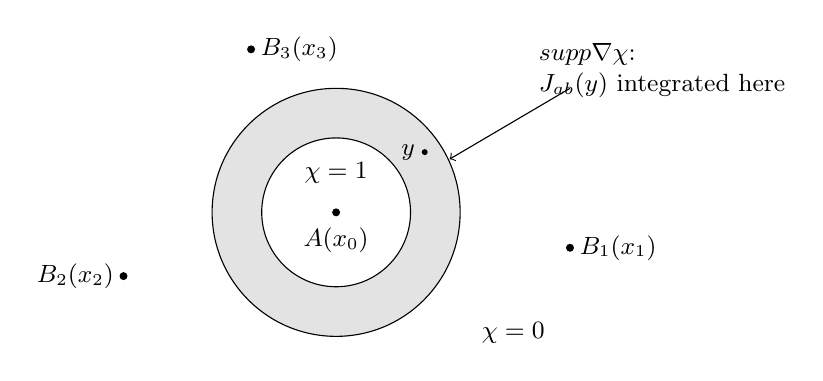
\begin{tikzpicture}[scale=0.9,font=\small]
\fill[gray!22,even odd rule] (0,0) circle (1.75) (0,0) circle (1.05);
\draw (0,0) circle (1.05); \draw (0,0) circle (1.75);
\fill (0,0) circle (1.6pt) node[below=2pt] {$A(x_0)$};
\node at (0,0.55) {$\chi=1$};
\fill (1.25,0.85) circle (1.2pt) node[left] {$y$};
\node[align=left] at (4.6,2.0) {$\operatorname{supp}\nabla\chi$:\\ $J_{ab}(y)$ integrated here};
\draw[->] (3.3,1.75) -- (1.6,0.75);
\fill (3.3,-0.5) circle (1.6pt) node[right] {$B_1(x_1)$};
\fill (-3.0,-0.9) circle (1.6pt) node[left] {$B_2(x_2)$};
\fill (-1.2,2.3) circle (1.6pt) node[right] {$B_3(x_3)$};
\node at (2.5,-1.7) {$\chi=0$};
\end{tikzpicture}
\caption{The shell flux of Definition~\ref{def:D13}. The cutoff~$\chi$ equals one near the insertion $A(x_0)$ and vanishes near the spectators $B_i(x_i)$; the current is integrated against $\nabla\chi$ on the shaded annulus. Conservation makes the flux independent of~$\chi$, so the annulus may shrink towards~$x_0$ or grow until it meets a spectator. It says nothing about flux through large spheres. The vanishing of the total angular flux at infinity is proved separately: on coordinate lines in Lemma~\ref{lem:G-collinear-flux}, and for all configurations in Lemma~\ref{lem:G3.1}.}
\label{fig:G-shell}
\end{figure}

The sign convention can be seen in one free example (Figure~\ref{fig:G-shell}). By Lemma~\ref{lem:G1.1}(iv), $\maxwellcorr_2(\curvaturesquare(x),\curvaturesquare(y))=c|x-y|^{-8}$ with $c=3\dimG/\pi^4$. The translation shell Ward identity~\eqref{eq:G-free-shells} and the free derivative law give, for a shell around~$x$,
\begin{equation*}
\mathcal P_b^{\maxwellstress}=\partial_{x_b}\bigl(c|x-y|^{-8}\bigr)=-8c\,(x_b-y_b)|x-y|^{-10}.
\end{equation*}
Replacing $\maxwellstress$ by $\lambda\maxwellstress$ multiplies this flux by~$\lambda$, so the requirement that the flux be the derivative fixes both the normalization and the sign of the stress tensor. This is a free-field calculation; nothing is asserted here about the form of interacting correlations.

The next lemmas concern only the invariant polynomial algebra of Definition~\ref{def:D11}, realized by the Taylor sections of Lemma~\ref{lem:A1}. A curvature jet of order~$j$ has weight~$j+2$. Let $\mathfrak P$ be the complex polynomial algebra on all on-shell jets, $\mathfrak P_{\le j}$ its subalgebra using orders at most~$j$, and $\mathfrak P^G$ the invariant subalgebra. The invariant polynomials of weight at most~$d$ identify with~$\maxwellspace{d}$. For a spectator degree~$d$ put
\begin{equation*}
\mathfrak N_d=\{P\in\mathfrak P:S^{\rm Max}(P(0),u_1(x_1),\ldots,u_n(x_n))=0
\text{ for all }n,\ u_i\in\maxwellspace{d},\ (0,x)\in\Conf{n+1}\},
\end{equation*}
with every polynomial Wick ordered at its own site. The degree of~$P$ is unrestricted. The next result says that spectators of one bounded degree detect every invariant polynomial, however high its jet order.
\begin{lemma}[Detection by bounded spectators]\label{lem:G-detection}
There is $d_0\in\N$ such that
\begin{equation}\label{eq:G-detection}
\mathfrak N_{d_0}\cap\mathfrak P^{G}=\{0\}.
\end{equation}
\end{lemma}
The proof has two stages. At a fixed jet order, finite generation and reflected positivity give a bound on the spectator degree. To make the bound independent of the jet order, a quadratic spectator isolates a highest-order jet derivative of~$P$ by its harmonic pole, and induction on weight removes that jet order.

The extraction rests on the difference between a single harmonic pole and a product of poles. In four dimensions $K(z)=\partial_1\partial_2|z|^{-2}=8z_1z_2|z|^{-6}$ is harmonic and homogeneous of degree $-4$; multiplication by $|z|^{4}$ leaves $8z_1z_2|z|^{-2}$, which is not analytic at zero, and only $|z|^{6}$ clears it. The product of two poles $|z|^{-2}\cdot|z|^{-2}=|z|^{-4}$ has the same degree but is already cleared by~$|z|^4$. In general a product of poles of orders $r_1,r_2\ge2$ is cleared by $|z|^{2(r_1+r_2-2)}$, while a harmonic pole of order $r_1+r_2$ needs $|z|^{2(r_1+r_2-1)}$.
\begin{proof}[Proof of Lemma~\ref{lem:G-detection}]
\emph{Step 1: bounded jet order.} Fix~$j$. The algebra~$\mathfrak P_{\le j}$ is a polynomial algebra on finitely many variables, hence Noetherian by the Hilbert basis theorem~\cite[Lemma~10.31.1]{Stacks2026}. Its ideal generated by invariant polynomials of positive ordinary degree therefore has finitely many invariant, ordinary-homogeneous generators~$f_\alpha$. Every invariant ordinary-homogeneous polynomial is a sum of products of invariant homogeneous polynomials of weight at most some~$b_j$: write $P=\sum a_\alpha f_\alpha$, keep only terms of total degree~$\deg P$, and replace $a_\alpha$ by its gauge average, whose degree is smaller; induction on the degree concludes.

Spectators of degree~$b_j$ detect: $\mathfrak N_{b_j}\cap\mathfrak P^G\cap\mathfrak P_{\le j}=\{0\}$. Otherwise take its lowest nonzero ordinary-homogeneous part~$P_r$ and split a product of homogeneous factors of total ordinary degree~$r$ into distinct nearby spectator sites. Every leg of~$P$ must pair with a spectator leg, so terms with internal spectator contractions, or with higher-degree parts of~$P$, vanish. As the spectator sites coalesce, Wick's rule gives the two-site pairing of~$P_r$ with their ordinary product. Each factor has weight at most~$b_j$, so for $P\in\mathfrak N_{b_j}$ this limit is zero. Choose the product sum to be the reflection of~$\overline{P_r}$; Lemma~\ref{lem:G1.1}(ii) makes this pairing strictly positive, a contradiction.

\emph{Step 2: pole extraction.} Put $g=\dimG$ and choose $d_0\ge\max\{b_g,2g+5\}$. In a real colour basis write $X_{j,\alpha}(p)$ for the jet coordinate tested by a scalar order-$j$ probe~$p$. For scalar probes~$p,q$ of orders $k,l$, the invariant quadratic $\sum_\alpha{:}X_{k,\alpha}(p)X_{l,\alpha}(q){:}$ has weight~$k+l+4$. Its collision with a polynomial using jets through order~$j$ has, in the coefficient where just the order-$k$ leg contracts at order~$j$, the polynomial
\begin{equation}\label{eq:G-collision}
\sum_\alpha X_{l,\alpha}(q)\sum_\mu
C_{k,j}(p,e_\mu;z)\frac{\partial P}{\partial X_{j,\alpha}(e_\mu)},
\end{equation}
where $(e_\mu)$ is a basis of order-$j$ probes and $C_{k,j}$ their differentiated curvature covariance.

\emph{Claim.} If $P\in\mathfrak N_{d_0}$, $l<k$ and $k+l+4\le d_0$, then~\eqref{eq:G-collision} lies in~$\mathfrak N_{d_0}$. Put $r=4+k+j$. Tested against fixed exterior spectators, the term~\eqref{eq:G-collision} is harmonic and homogeneous of degree~$-r$ in~$z$, so $|z|^{2(r-1)}$ times it is analytic at zero. The other terms, expanded in Taylor series at each singular order, give at order~$r$ homogeneous functions that become analytic after multiplication by $|z|^{2(r-2)}$: a double contraction is a product of poles of orders $r_1,r_2\ge2$, cleared by $|z|^{2(r_1+r_2-2)}$, and Taylor terms keep this improvement. The contraction of the order-$l$ leg alone has order at most $4+l+j<r$. The claim now follows from:
\begin{equation*}
\text{a harmonic $K$, homogeneous of degree $-r\le-2$, with $|z|^{2(r-2)}K$ analytic at $0$, vanishes.}
\end{equation*}
Indeed $\Delta(|z|^{2s}K)=4s(s+1-r)|z|^{2s-2}K$ in four dimensions; successive Laplacians show that~$K$ extends analytically, and negative homogeneity makes it zero. Expand the collision through an order exceeding $8+k+l+2j$. Since its correlation with the quadratic test and further bounded-degree spectators vanishes identically, comparing successive radial homogeneities makes the order-$r$ harmonic pole zero, so~\eqref{eq:G-collision} belongs to~$\mathfrak N_{d_0}$.

\emph{Step 3: induction on weight.} Take $k=g+1$ and $l=0,\ldots,g-1$. For each~$l$ choose a probe~$q_l$ and a jet value~$v_l$ with $q_l(v_l)=1$. The matrix $(X_{l,\alpha}(q_l))_{l,\alpha}$ has nonzero polynomial determinant: assigning~$v_l$ to colour~$l$ and zero to the other colours in order~$l$ makes it the identity. For $j>g$ the polynomial~\eqref{eq:G-collision} replaces an order-$j$ jet by an order-$l$ jet, so its weight is smaller, and the induction hypothesis makes it zero. Multiplication by the transposed cofactor matrix shows that every one-colour contraction in~\eqref{eq:G-collision} vanishes. As $z,p$ vary, the forms $C_{k,j}(p,\cdot;z)$ span the dual of the order-$j$ jets: their common annihilator generates a Maxwell wave whose order-$k$ jets vanish everywhere, a polynomial of degree below~$k$ with negative homogeneity, hence zero, and~\eqref{eq:G-kelvin} makes the probe zero. Hence every order-$j$ partial derivative of~$P$ vanishes. Descending from the top order removes all orders above~$g$; Step~1 with spectator bound~$b_g$ treats the rest.
\end{proof}

Let $\mathcal C_d$ be the real space of complex linear tuples $\mathsf X_a:\maxwellspace{d}\to\maxwellspace{d+1}$ that commute with conjugation, kill the unit, are vector-covariant under~$\hypercubic$, and send $\maxwellspace{e}$ into~$\maxwellspace{e+1}$ for $e\le d$. For $\mathsf X\in\mathcal C_d$ the Ward sum is
\begin{equation*}
\mathcal E_b(\mathsf X;\boldsymbol u,x)=\sum_i S_n^{\rm Max}(u_1,\ldots,\mathsf X_bu_i,\ldots,u_n;x).
\end{equation*}
Finitely many tests on lines determine its kernel.
\begin{lemma}[Finite vector Ward tests]\label{lem:G1-vector}
For all sufficiently large~$d$, finitely many positional derivatives of $\mathcal E_b(\mathsf X;\boldsymbol u,x)$, with $u_i\in\maxwellspace{d}$ and~$x$ on a coordinate line perpendicular to~$e_b$, define a real linear map~$\mathcal T_d$ with
\begin{equation}\label{eq:G-free-tests}
\ker\mathcal T_d=\R\partial^{\rm Max}\quad\text{in }\mathcal C_d.
\end{equation}
\end{lemma}
\begin{proof}
Take $d\ge d_0$ from Lemma~\ref{lem:G-detection}. Suppose all the stated jets of the Ward sums of~$\mathsf X$ vanish.

\emph{Step 1: continuation off the lines.} Free correlations are real analytic off the diagonals by~\eqref{eq:G-curvature}, so every Ward sum vanishes near each testing line. For a separated configuration choose distinct ordered line coordinates respecting the strict order of its coordinates in that axis. The straight segment to the line configuration stays separated: strict inequalities persist, and coordinate ties are separated by the line coordinates. Analytic continuation along it gives $\mathcal E_b=0$ on~$\Conf{n}$.

\emph{Step 2: weight four.} Let $\mathsf J_j$ be the scalar on-shell order-$j$ jet space. For $p\in\mathsf J_0^*$ put $U(p)=\sum_\alpha{:}X_{0,\alpha}(p)^2{:}$. Simplicity, the filtration and inversion parity force $\mathsf X_bU(p)$ to be a colour contraction of one order-zero and one order-one jet, represented by a linear map $A_p:\mathsf J_0\to\mathsf J_1^*$. In the Ward identity of $U(p),U(q),U(w)$ let the first two points coalesce along~$tu$ and multiply by~$t^5$. The term with $\mathsf X_b$ at the distant point tends to zero, and the two remaining triangular Wick contractions give, for every $X\in\mathsf J_0$ and with $C_{1,0}$ taken in one colour,
\begin{equation*}
C_{1,0}(A_pX,q;u)\,q(X)=C_{1,0}(A_qX,p;u)\,p(X).
\end{equation*}
Arbitrary~$X$ are reached by choosing the distant probe~$w$ through the invertible order-zero covariance~\eqref{eq:G-kelvin}. If $p(X)=0$, choose $q(X)\ne0$; varying $q,u$ gives $A_pX=0$. Thus $A_pX=p(X)f_bp$, and the same identity shows that $f_b:\mathsf J_0^*\to\mathsf J_1^*$ is real linear with $C_{1,0}(f_bp,q;u)=C_{1,0}(f_bq,p;u)$.

\emph{Calculation of~$f_b$.} Write $e^{ij}$ for the curvature coordinate and $\partial_he^{ij}$ for its first jet. For $f_1e^{12}$, sign parity permits only $\partial_1e^{12},\partial_3e^{23},\partial_4e^{24}$; interchange of axes~$3,4$ and $\sum_i\partial_ie^{i2}=0$ reduce their span to $\R\partial_1e^{12}$. For $f_1e^{23}$ the candidates $\partial_1e^{23},\partial_2e^{13},\partial_3e^{12}$ reduce, by antisymmetry in axes~$2,3$ and Bianchi, to $\R\partial_1e^{23}$. Permutations leave two constants, which agree because $C_{1,0}(\partial_1e^{12},e^{23};e_1+e_3)=-1/(2\pi^2)\ne0$ by~\eqref{eq:G-curvature}. Therefore $f_b=c_{\rm jet}\partial_b$, and since $\partial_bU(p)$ has two identical terms, $\mathsf X_b=c\,\partial^{\rm Max}_b$ on weight four with $c=c_{\rm jet}/2$.

\emph{Step 3: higher weights.} Set $\mathsf X^\circ_b=\mathsf X_b-c\,\partial^{\rm Max}_b$. Translation invariance makes its Ward sums zero, and it kills every free stress component. Insert into such a sum a free stress shell for the dilation field $v(y)=y-x_0$, surrounding only the distinguished point. The term where $\mathsf X^\circ_b$ acts on the stress is zero. The other shell terms are given by the polarized calculation in Lemma~\ref{lem:G1.1}, now with this~$v$; the extra derivative of~$v$ contracts with the trace of the free stress, which is zero by~\eqref{eq:G-free-tensor}. The local Lie derivative of a two-form under dilation is $y\cdot\nabla+2$, and on jets it gives the weight operator $\mathsf D^{\rm wt}X_{j,\alpha}=(j+2)X_{j,\alpha}$. Subtracting the Ward sum with distinguished label~$\mathsf D^{\rm wt}u$ shows $[\mathsf D^{\rm wt},\mathsf X^\circ_b]u\in\mathfrak N_d$, and Lemma~\ref{lem:G-detection} makes it zero. So $\mathsf X^\circ_b$ preserves each weight. Inversion acts there by~$(-1)^{\rm weight}$, whereas vector covariance makes $\mathsf X^\circ_b$ odd under inversion; hence $\mathsf X^\circ_b=0$.

\emph{Step 4: finite selection.} Conversely translation invariance annihilates every test on~$\partial^{\rm Max}$. The real space~$\mathcal C_d$ is finite-dimensional; successively choose a test nonzero on the current kernel modulo this line. Each choice lowers its dimension, so finitely many tests have precisely the asserted kernel.
\end{proof}

The internal tests rest on one elementary fact about the plane generators $K_{ab}=E_{ba}-E_{ab}$ of $\mathfrak{so}(4)$. Call a coordinate quarter turn the rotation $e_a\mapsto e_b$, $e_b\mapsto-e_a$ in one coordinate plane.
\begin{lemma}[Alternating planes]\label{lem:G-planes}
Let $\beta:\mathfrak{so}(4)\times\mathfrak{so}(4)\to V$ be real bilinear and alternating, with $\beta(hKh^{-1},hLh^{-1})=\beta(K,L)$ for every coordinate quarter turn~$h$. Then $\beta=0$.
\end{lemma}
\begin{proof}
The quarter turns generate the determinant-one signed permutations: they project onto the transpositions of $S_4$, and squares of quarter turns give the diagonal sign changes with two minus signs. Conjugation by a diagonal sign matrix~$s$ multiplies $K_{ab}$ by $s_as_b$; conjugation by a permutation matrix permutes the planes. \emph{Overlapping planes:} $s=\operatorname{diag}(1,1,-1,-1)$ fixes $K_{12}$ and reverses the sign of $K_{13}$, so $\beta(K_{12},K_{13})=-\beta(K_{12},K_{13})=0$. \emph{Disjoint planes:} the even permutation $(13)(24)$ interchanges $K_{12}$ and $K_{34}$, so $\beta(K_{12},K_{34})=\beta(K_{34},K_{12})=-\beta(K_{12},K_{34})=0$. Every pair of distinct planes is carried to one of these two pairs by a signed permutation of determinant one, and $\beta(K,K)=0$; bilinearity gives $\beta=0$.
\end{proof}

Let $\mathcal B_d$ consist of alternating real-bilinear families $\Delta:\mathfrak{so}(4)^2\to\operatorname{End}_{\C}\maxwellspace{d}$ which commute with conjugation, kill the unit, preserve every lower-degree subspace, and satisfy
\begin{equation*}
R^{\rm Max}(h)\Delta(K,L)=\Delta(hKh^{-1},hLh^{-1})R^{\rm Max}(h)
\qquad(h\in\hypercubic,\ \det h=1).
\end{equation*}
The next result removes the defect in the rotation commutator.
\begin{lemma}[Finite internal Ward tests]\label{lem:G1-internal}
For every $d\ge4$, finitely many sums
\begin{equation}\label{eq:G-erasure-test}
\sum_i S_n^{\rm Max}(u_1,\ldots,\Delta(K,L)u_i,\ldots,u_n;x),
\qquad u_i\in\maxwellspace{d},\quad x\in\Conf{n},
\end{equation}
separate~$\mathcal B_d$.
\end{lemma}
\begin{proof}
Suppose all these sums vanish and fix $\mathsf Z=\Delta(K,L)$. On the weight-four space let $b_x(u,v)=S_2^{\rm Max}(u,v;x,0)$. The order-zero Kelvin formula and Wick's rule give $b_x(u,v)=b_y(R^{\rm Max}(\mathcal R_y\mathcal R_x)u,v)$ for $|x|=|y|\ne0$. Both $\mathsf Z$ and the orthogonal action preserve this space. Applying $b_x(\mathsf Zu,v)+b_x(u,\mathsf Zv)=0$ at~$x$ and~$y$, and nondegeneracy of~$b_y$, shows that~$\mathsf Z$ commutes with $R^{\rm Max}(\mathcal R_y\mathcal R_x)$, in particular with every coordinate quarter turn. With the signed covariance of~$\Delta$, the function $(K,L)\mapsto\Delta(K,L)u$ satisfies the hypothesis of Lemma~\ref{lem:G-planes} for each weight-four~$u$, so~$\mathsf Z$ vanishes on weight four, including the stress.

Insert a free angular stress shell around the distinguished point only, as in Step~3 of the proof of Lemma~\ref{lem:G1-vector}. Subtracting the Ward sum with the angularly differentiated label gives $[\mathsf L^{\rm Max}(M),\mathsf Z]u\in\mathfrak N_d$. This polynomial has weight at most~$d$, so Lemma~\ref{lem:G1.1}(ii) makes it zero. Hence $\mathsf Z$ commutes with all infinitesimal rotations, and differentiating $e^{t\mathsf L(M)}\mathsf Z-\mathsf Ze^{t\mathsf L(M)}$ gives commutation with coordinate quarter turns in every degree. Lemma~\ref{lem:G-planes} again gives $\Delta=0$. Finite-dimensionality selects a finite separating subfamily by successively reducing the common kernel.
\end{proof}

\subsection{Lattice inputs}\label{sec:G-lattice}

The insertions are those of Definition~\ref{def:D08}, with coefficient polynomials from Definition~\ref{def:D19} and Lemma~\ref{lem:A1}. The inverse coefficient estimate of Lemma~\ref{lem:E-marked-step} inverts the marked coefficient map; the corrected sources and normalized integral of Lemmas~\ref{lem:E-Gaussian-sources} and~\ref{lem:E-source-integral} bound the remainders; the uniform displacement estimate of Lemma~\ref{lem:E-displacement} controls positions, with coordinate separations at least four times the displacement margin. Chessboard seminorms are those of Definition~\ref{def:D27}. Cutoff limits are taken in the order~\eqref{eq:E2-tails}, followed by the fixed extraction of Lemma~\ref{lem:F1}; an ordered limit point of a bounded coefficient family is its limit along an ultrafilter containing the ordered tails.

Fix arity and degree bounds $n\ge2,D\ge1$ and $R\ge1$. A basis word is a list of members of fixed real bases of $\maxwellspace{d}$, $d\le D$. Put
\begin{equation*}
K_{R,m}=\{x:|x|\le R,\ \sepinf(x)\ge R^{-1}\},\qquad
E_\delta=\{x:|x_i^a-x_j^a|>\delta\ (i\ne j,\ a=1,\ldots,4)\}.
\end{equation*}
The comparison exponents $\alpha_0,\alpha_1,\alpha_2>0$ and $c<0$ have the following roles: $\alpha_0$ sets the comparison radius, $\alpha_1$ the cells used for moment bounds, $\alpha_2$ the smaller cells used for displacement bounds, and~$c$ the width of the excluded coordinate strips. They satisfy
\begin{equation}\label{eq:G-exponents}
\alpha_1+6<\alpha_0,\quad \alpha_2+5<\alpha_0+c,\quad
(\alpha_0-\alpha_1)Dn+c<0,\quad
(\alpha_0-\alpha_2)Dn-\alpha_0-c<0.
\end{equation}
The first two inequalities place the chessboard cells; the last two make the excluded strips negligible. One explicit choice, with $n_{\max}=\max(n,D)$, is $\kappa_1=7n_{\max}(n_{\max}+2)+1$, $\kappa_2=6+\kappa_1$, $\alpha_0=17+n_{\max}+\kappa_1+\kappa_2n_{\max}(n_{\max}+2)+\kappa_2$, $\alpha_1=\alpha_0-7$, $\alpha_2=\alpha_0-\kappa_2$ and $c=-\kappa_1$. Write $M_k=\cutoffsize_k$ and set
\begin{equation}\label{eq:G-balance}
r_k=a_kM_k^{\alpha_0},\qquad \mathfrak s_k=M_k^{-\alpha_0},\qquad
\delta_k=M_k^{c},\qquad
R^{\rm cell}_k=CM_k^{(\alpha_0-\alpha_1)D},\quad R^{\rm var}_k=CM_k^{(\alpha_0-\alpha_2)D},
\end{equation}
where $C\ge1$ depends only on $n,D,R$ and the construction and is fixed in the proof of Lemma~\ref{lem:G-lattice}. Thus $r_k\mathfrak s_k=a_k$: the normalized grid is the physical construction grid. For an ordered limit point $c_{k,d}:\maxwellspace{d}\to V_d$ of the lifts in Lemma~\ref{lem:G-lattice}, and the quotient $\pi_d:V_d\to F_d$ of Definition~\ref{def:D10}, define the rescaled correlation
\begin{equation*}
S^{\rm sc}_k(\boldsymbol u;x)=S_m(\pi_{d_i}c_{k,d_i}u_i;r_kx).
\end{equation*}

The following comparison uses one coefficient family for every word within the fixed bounds. Its constants may depend on these bounds, the word and the construction. The arity, degree and radius bounds are fixed first, then the level and the lifts; the estimates then hold for every basis word within these bounds.
\begin{lemma}[Lattice comparison at small radii]\label{lem:G-lattice}
There are arbitrarily large levels~$k$, real $\hypercubic$-equivariant lifts $\Lambda_{k,N,p,d}:\maxwellspace{d}\to V_d$ preserving the degree-zero unit, and $\varepsilon_k\to0$ such that every ordered limit point of these lifts satisfies, for every basis word with $m\le n$,
\begin{equation}\label{eq:G-lattice-input}
\begin{aligned}
|S^{\rm sc}_k|&\le (R^{\rm cell}_k)^m &&\text{on }K_{R,m},\\
\|\nabla S^{\rm sc}_k\|&\le4m (R^{\rm var}_k)^m/\delta_k &&\text{on }K_{2R,m}\cap E_{4\delta_k},\\
|S^{\rm sc}_k-S_m^{\rm Max}|&\le\varepsilon_k
&&\text{on }(\mathfrak s_k\Z)^{4m}\cap K_{2R,m}\cap E_0.
\end{aligned}
\end{equation}
At fixed~$k$ the lifts are bounded on ordered tails.
\end{lemma}
The lifts are chosen so that the rescaled insertions have the free Wick polynomials as Gaussian leading part~\eqref{eq:G-lift-equation}. A subset recursion removes the continuum Gaussian moments; for exact Gaussian variables each remainder has mean zero, and the source estimates of Section~\ref{sec:partII-E} make each remainder small in chessboard seminorm~\eqref{eq:G-source-root}. The chessboard inequality then gives the comparison on the grid, and the coarser normalizations $\alpha_1,\alpha_2$ give the size and gradient bounds off the grid.
\begin{proof}
\emph{Step 1: lifts.} Choose a real $\hypercubic$-equivariant polynomial representative map $\iota_d^{\rm free}$ for the on-shell quotient, using the Taylor sections of Lemma~\ref{lem:A1} and averaging a real splitting over~$\hypercubic$. Let $\mathsf C_{k,N,p,d}$ be the marked coefficient map from level~$k$ down to~$\reflevel{d}$, after the Wick-ordering correction of Lemma~\ref{lem:E-source-polynomial}. Write $\delta_t^{\rm wt}$ for multiplication of a weight-$j$ monomial by~$t^j$; the factor-count scaling~$t^{\factorcount}$ is that of Definition~\ref{def:D08}. The Gaussian field divided by the small-field threshold has scale
\begin{equation*}
\mathfrak t_{k,N,p}=(t_k\sqrt{\beta_{N,p,k}})^{-1},\qquad
0<\mathfrak t_{k,N,p}^{-1}\le2M_k,
\end{equation*}
since $t_k=M_k/\sqrt{\refbeta_k}$ is the small-field threshold of Part~I and $\beta_{N,p,k}\le2\refbeta_k$. Solve
\begin{equation}\label{eq:G-lift-equation}
\mathsf C_{k,N,p,d}\Lambda_{k,N,p,d}u
=\mathfrak t_{k,N,p}^{-\factorcount}\delta_{M_k^{\alpha_0}}^{\rm wt}\iota_d^{\rm free}u.
\end{equation}
The solution exists and obeys
\begin{equation}\label{eq:G-lift-bound}
|v|_1\le K_{k,d}a_k^d|\mathsf C_{k,N,p,d}v|_1,
\end{equation}
with $K_{k,d}$ independent of~$N,p$ at fixed~$k$. Indeed, apply the inverse estimate of Lemma~\ref{lem:E-marked-step} at each step $m+1\to m$ from level~$k$ down to~$\reflevel{d}$, and the coefficient comparison in the proof of Lemma~\ref{lem:E-source-polynomial}, whose relative error is less than~$1/4$, so its inverse costs at most~$2$. One may take $K_{k,d}$ to be twice the product of the finitely many column and block factors up to~$k$, enlarged by the fixed basis norms. The coefficient map is injective, hence invertible on its finite coefficient space, and its unit, conjugation and signed laws pass to the inverse. The bound on~$\mathfrak t^{-1}$ bounds the right side at fixed~$k$, so the lifts are bounded on cutoff tails.

\emph{Step 2: subset recursion.} Lemmas~\ref{lem:E-source-polynomial}--\ref{lem:E-source-integral} hold for an arity bound~$n\ge2$, at most~$n$ marks per cell and any compact position set with positive point separation; apply them to the interval~\eqref{eq:E-window} with exponent~$\alpha_0$ and position set~$K_{2R,m}$. Their covariance and Taylor bounds are uniform on $K_{2R,m}$, whose point separations are at least $(2R)^{-1}$, and need no lower bound on coordinate differences; only the reflected placement below requires~$E_0$. Write $I_i=O_{N,p}^{(d_i)}(\Lambda_{k,N,p,d_i}u_i,r_kx_i/a_N)$ at compatible lattice points. For a subset~$J$ put $G_J=S_{|J|}^{\rm Max}((u_i)_{i\in J};(x_i)_{i\in J})$ and define
\begin{equation*}
R_\varnothing=1,\qquad
R_I=\prod_{i\in I}I_i-\sum_{\varnothing\ne J\subseteq I}G_JR_{I\setminus J}.
\end{equation*}
This subtracts the full continuum Gaussian moment on every subset of slots; for exact continuum Gaussian variables its nonempty coefficients have expectation zero, by induction on~$|I|$. The Wick-ordering correction and~\eqref{eq:G-lift-equation} identify the leading Gaussian correlations with these continuum moments at the normalized grid points, as calculated in Lemma~\ref{lem:E-source-polynomial}. Covariance, Taylor and localization errors remain in the regular and forced source terms.

\emph{Step 3: chessboard seminorm of the remainders.} The finite-set clause of Lemma~\ref{lem:E1.1} gives arbitrarily late common terminal levels~$k$ for the three exponents $\alpha_0,\alpha_1,\alpha_2$. Use the interval~\eqref{eq:E-window} with exponent~$\alpha_0$, its width level $w_{\alpha_0}(k)=k-h_k(\alpha_0)-v_k$ and its centered tiling $\mathcal C^{\rm tile}_{w_{\alpha_0}(k)}(0)$. Put $q_k=\log M_k/(16n)$ and give each mark weight $e^{2q_k}\le M_k^{1/16}$. The weighted mode norm in the proof of Lemma~\ref{lem:E-replication} multiplies mark weights over subsets, so coefficient extraction for a nonempty~$I$ contributes $e^{-2q_k|I|}$ in each reflected cell, and the corrected-source iteration of Lemma~\ref{lem:E-Gaussian-sources} keeps this mark weight on the selected comparison intervals. Work in $\C[z_1,\ldots,z_m]/(z_i^2)$ and multiply by the reciprocal of the continuum free moment polynomial; its coefficient of~$z_I$ is exactly~$R_I$. After the finite Gaussian contractions on every subset, the remaining source modes have zero leading Gaussian coefficient. In the source iteration, terms linear in these modes cost the finite stage constant, and every other connected term contains at least two residual modes and is bounded by their squared norm times a fixed power of~$M_k$; this is~\eqref{eq:E-source-step}. The covariance and localization errors of Lemma~\ref{lem:E-source-polynomial} are below the corresponding source tolerance at entry~\eqref{eq:E-source-iteration}. Lemma~\ref{lem:E-Gaussian-sources}, applied to the coefficients~\eqref{eq:E-corrected-coefficients} of these finitely many subset modes, gives this mark weight with constants depending only on $n,D,R$ and the construction; its sums are rooted at a mark and do not count the replicated cells.

The normalized positive integral costs, per cell, at most the stage constant $Q_{J_k}^{\rm cmp}$ of~\eqref{eq:E-comparison-cost} (Lemma~\ref{lem:E-source-integral}), which contains the term $1+n$ for at most~$n$ marks. Item~\ref{it:E-entries} imposes $Q_j^{\rm cmp}\le\log M_t/(16n)$ for each arity bound, hence $Q_{J_k}^{\rm cmp}\le q_k$; the entry is chosen after the finitely many source constants. Taking the root over the reflected cells gives
\begin{equation}\label{eq:G-source-root}
\|R_I\|_{\mathcal C^{\rm tile}_{w_{\alpha_0}(k)}(0)}
\le e^{q_k-2q_k|I|}\le M_k^{-1/(16n)}
\qquad(\varnothing\ne I\subseteq\{1,\ldots,m\}).
\end{equation}
The smallness comes from the corrected density at large coupling: its source terms stay bounded at a growing mark weight, while the unmarked normalization grows more slowly than that weight. The estimate concerns the complete reflected array, before absolute values are taken, and needs no independence of the insertions.

\emph{Step 4: comparison on the grid.} Distinct coordinate differences at normalized grid points are at least $\mathfrak s_k$, so their physical differences are at least~$a_k$. The reading map assigns the corresponding level-$k$ sites without rounding, and the interval margin~\eqref{eq:E-window-geometry} contains the inspected stencils and their reflected copies. Expanding the recursion, applying~\eqref{eq:E-chess} to each~$R_I$ and bounding the free submoments on~$K_{2R,m}$ gives $C_{R,\boldsymbol u}M_k^{-1/(16n)}$, the last line of~\eqref{eq:G-lattice-input}.

\emph{Step 5: size and variation off the grid.} At its own normalization the singleton comparison gives a chessboard seminorm at most $1+|S_1^{\rm Max}(u)|$. For exponent~$\alpha_1$, changing normalization to~$M_k^{\alpha_0}$ multiplies a weight-$j$ coefficient by $M_k^{(\alpha_0-\alpha_1)j}$, so the finite coefficient sum bounds these seminorms by~$R^{\rm cell}_k$ for~$C$ large; exponent~$\alpha_2$ gives~$R^{\rm var}_k$. Include every reflected basis label and its complex conjugation in these maxima. The two interval lengths of~\eqref{eq:E-window} give, with the stage block ratio~$L$,
\begin{equation}\label{eq:G-root-sides}
\frac{a_{w_b(k)}}{a_k}=L^{h_k(b)+v_k}
\le L^2M_k^{b+2}B_k^{10}\le M_k^{b+5}
\qquad(b=\alpha_1,\alpha_2),
\end{equation}
after the stage entry, where $L$ is fixed and $B_k=M_k^{o(1)}$. So the $\alpha_1$ cell is at most $a_kM_k^{\alpha_1+6}=o(r_k)$ and the $\alpha_2$ cell is $o(r_k\delta_k)$ by~\eqref{eq:G-exponents}. The chessboard inequality bounds separated continuum moments by~$(R^{\rm cell}_k)^m$. The physical diameter on~$r_kK_{2R,m}$ is at most $4Rr_k<L_p/2$ on the ordered tails, so the torus separation~$g_p$ of Lemma~\ref{lem:E-displacement} is the minimum ordinary coordinate separation, which exceeds $4r_k\delta_k$ on~$E_{4\delta_k}$. The uniform clause of Lemma~\ref{lem:E-displacement}, with margin $r_k\delta_k$ and the reflected seminorms included in~$R^{\rm var}_k$, gives $4m(R^{\rm var}_k)^m/\delta_k$ after rescaling. The three normalizations use the same coefficient map and lifts and the same terminal levels; the finitely many cutoff tails can be intersected.

\emph{Step 6: limits.} Take any ordered limit point of the bounded lifts. Lemma~\ref{lem:E3.1} and~\eqref{eq:F-conf} pass the moment estimates to the fixed table, and Proposition~\ref{prop:FC} with Lemma~\ref{lem:F2} passes the difference bound. No extraction of the table or the volume sequence is made.
\end{proof}

For the shell estimate take $\varkappa\in\{0,1\}$, $A\in F_d$, $B\in F_4$ and $D=d+1-\varkappa$. The shell factor has scaling degree $3+\varkappa$: integration over four dimensions contributes four powers of the radius, the differentiated cutoff removes one, and the constant or linear vector field contributes~$\varkappa$. Since the two inserted fields have total degree $d+4$, the expected output degree is $(d+4)-(3+\varkappa)=D$. A grid test is a separated configuration $(0,x_i)$ on $a_{j_0}\Z^4$ for some level~$j_0$, generic in each coordinate, with a fixed spectator list~$\boldsymbol B_i$. Its response functional and marked response are
\begin{equation*}
\mathsf r_i(v)=S(v(0),\boldsymbol B_i(x_i)),\qquad
\mathfrak h_i(y)=S(B(y),A(0),\boldsymbol B_i(x_i)).
\end{equation*}
Finite collections may use different grids, and the union of all these configurations is dense. The next lemma shows that every finite combination of tests annihilating $F_D$ also annihilates the limiting shell response.
\begin{lemma}[Annular annihilator estimate]\label{lem:G-annular}
For every finite list of grid tests and coefficients $g_i\in\C$ with $\sum_i g_i\mathsf r_i=0$ on~$F_D$, there are $\rho_l\downarrow0$ such that
\begin{equation}\label{eq:G-annular-input}
\sup_{1/4\le|z|\le2}\left|\sum_i g_i\rho_l^{3+\varkappa}\mathfrak h_i(\rho_lz)\right|\longrightarrow0.
\end{equation}
\end{lemma}
\begin{proof}
The local sections of Lemma~\ref{lem:A1} and Lemmas~\ref{lem:E2.2}--\ref{lem:E2.3} represent the product of two nearby marked insertions by one marked insertion of degree~$D$; Proposition~\ref{prop:FC} and Lemma~\ref{lem:F2} pass to the quotient. Put $h=3+\varkappa$, so $D+h=d+4$. Recall $s_m=\log(a_m^{-1})$ from~\eqref{eq:I12-levels}. Use the support radius $B_m=\lceil(\log\refbeta_m)^2\rceil$ of Part~I and take $\rho_m=128B_{m+1}^2a_{m+1}$, so $\log\rho_m=-s_m+o(s_m)$.

\emph{Step 1: two-mark representation.} Fix a centered cell around the distinguished point, disjoint from all spectator stencils, and a finer stopping level~$k_0\ge\reflevel{D}$ at which its replicated source estimate applies. Choose levels~$j(m)$ with
\begin{equation*}
\frac{s_{j(m)}}{s_m}\longrightarrow t=1+\frac1{64(d+12)};
\end{equation*}
they exist since $s_{m+1}/s_m\to1$ (Lemma~\ref{lem:E1.1}). At a grid point $y\in a_{j(m)}\Z^4$ with $\rho_m/16<|y|<4\rho_m$, choose representatives $a\in V_d,b\in V_4$ of~$A,B$, block their two marked insertions at~$y,0$ together, and retain the Taylor terms of weight at most~$D$. Their coefficient vector~$c_{N,p}(y)\in V_D$ is chosen by inverting the marked coefficient map. The exact difference is
\begin{equation*}
\rho_m^h O_{N,p}^{(4)}(b,y/a_N)O_{N,p}^{(d)}(a,0)
 -O_{N,p}^{(D)}(c_{N,p}(y),0).
\end{equation*}
Let $u_{m,1},u_{m,2}$ be the available mark weights of the degree-$d$ and rescaled degree-four marks at level~$j(m)$. The one-mark bounds, including~$\rho_m^h$, give $\log u_{m,1}=(-dt+o(1))s_m$ and $\log u_{m,2}=(-4t+h+o(1))s_m$; support weights, coefficient columns and threshold powers have logarithm~$o(s_m)$ by~\eqref{eq:E-marker-scales} and~\eqref{eq:E-log-cost}. Transporting each source to level~$m+1$ adds the volume factor $(a_{j(m)}/a_{m+1})^4$ to its weight. So the joint weight~$v_m$ and the dimensionless coefficient bound~$e_m$ of its Taylor remainder satisfy
\begin{equation}\label{eq:G-annular-cost}
\log v_m=[-D-(d+12)(t-1)+o(1)]s_m,\qquad
e_m\le\exp\{[(d+12)(t-1)+o(1)]s_m\}.
\end{equation}
Indeed the transported exponents sum to $-(d+4)t+h+8(1-t)=-D-(d+12)(t-1)$, and Taylor extraction costs the reciprocal joint weight times~$a_{m+1}^D$, which cancels the~$D$ term. This is the two-mark use of the source representation~\eqref{eq:E-source-form}, retaining its forced terms and their eligibility tests.

\emph{Step 2: backward matching.} Apply~\eqref{eq:E-backward-match-level} from~$m+1$ to the fixed stopping level~$k_0$. The matched remainder gains $\prod_{i=k_0}^{m}\ell_i^{1/8}=e^{(s_{m+1}-s_{k_0})/8}\ge e^{(s_m-s_{k_0})/8}$ in its inverse bound. Put $c_m=e^{s_m/32}$ and multiply the source by~$c_m$; its size is then at most
\begin{equation*}
c_me_me^{-(s_m-s_{k_0})/8}
\le\exp\{[-5/64+o(1)]s_m\},\qquad
\tfrac1{32}+(d+12)(t-1)-\tfrac18=-\tfrac5{64},
\end{equation*}
which eventually fits every fixed source allowance at~$k_0$. The residual-source estimate~\eqref{eq:E-residual-root} at the fixed cell and level~$k_0$ then bounds the chessboard seminorm of the unamplified residual by~$2C/c_m$, with~$C$ independent of~$m,N,p$. The inverse estimate~\eqref{eq:G-lift-bound} in degree~$D$ bounds~$c_{N,p}(y)$ on cutoff tails for each fixed~$m,y$. Interior support follows from $32\rho_m\to0$ and the support diameter $a_{m+1}(B_{m+1}^2+1+2048B_{m+1}^2)\to0$.

\emph{Step 3: cancellation at grid points.} Pass to an ordered limit point~$c(y)$ and project it to~$F_D$. The chessboard inequality~\eqref{eq:E-chess} for the residual and the fixed exterior stencils gives, simultaneously for the finite tests,
\begin{equation*}
|\rho_m^h\mathfrak h_i(y)-\mathsf r_i(\pi_Dc(y))|\le C_i c_m^{-1},
\end{equation*}
with the same coefficient vector for every spectator. Multiplication by~$g_i$ and summation cancel the response term, so $f_m(y)=\sum_i g_i\rho_m^h\mathfrak h_i(y)$ is $O(c_m^{-1})$ at all grid points of the enlarged annulus whose four coordinates are nonzero.

\emph{Step 4: interpolation across coordinate planes.} For a derivative order~$q$, Proposition~\ref{prop:FC} replaces the moving label by one of degree $4+q$. The centered and reflected bounds of Lemmas~\ref{lem:E2.3} and~\ref{lem:E-replication}, with~\eqref{eq:E-chess}, bound a field of fixed degree~$e$ by $\exp[(e+2+o(1))s_m]$, with a field-dependent constant of logarithm~$o(s_m)$. The finitely many later levels required for the fixed spectator word have logarithmic scale $s_m+o(s_m)$. Choose degree bounds~$e_{ij}$ for the spectator labels and put $C_0=8+d+\max_i\sum_j(e_{ij}+2)$. Since $\rho_m^h\le1$,
\begin{equation}\label{eq:G-annular-derivatives}
|\partial_a^q f_m(y)|\le \exp[(q+C_0+o(1))s_m]
\qquad(\rho_m/16<|y|<4\rho_m),
\end{equation}
with $C_0$ independent of~$q$. Choose $q$ with $q(t-1)>C_0$; since $a_{j(m)}=\exp[-(t+o(1))s_m]$, the $q$th derivatives along grid-sized segments tend to zero. On each coordinate segment of length $4(2^q+2)a_{j(m)}$ choose $q$ grid nodes with nonzero coordinates, mutually separated by at least $a_{j(m)}$. Lagrange interpolation gives $|g|\le C_q(\max_{\rm nodes}|g|+a_{j(m)}^q\sup|\partial^qg|)$ on the segment, with $C_q$ independent of~$m$. Apply it to ${\rm Re}\,f_m$ and ${\rm Im}\,f_m$ in each of the four axes; the segments stay in the enlarged annulus since $4(2^q+2)a_{j(m)}=o(\rho_m)$. Four successive interpolations give $\sup_{\rho_m/4\le|y|\le2\rho_m}|f_m(y)|\to0$. Select a decreasing subsequence of~$\rho_m$; it depends on the fixed tests and~$g$, as allowed.
\end{proof}

\subsection{Free comparison and the conserved line}\label{sec:partII-G.2}

The next lemma converts Lemma~\ref{lem:G-lattice} into the comparison of Part~I, measured uniformly over the supremum-norm unit ball of tests. No volume refinement is needed.
\begin{lemma}[Stable weak comparison]\label{lem:G2.1}
There is one stable scaling sequence such that, for every arity~$n$, degree list, $u_i\in\maxwellspace{d_i}$ and compact $\mathcal K\subset\Conf{n}$,
\begin{equation*}
\sup_{\|f\|_\infty\le1,\ \operatorname{supp}f\subset\mathcal K}\left|\int f(x)\bigl[S_n(\scaleframe{k}{d_i}u_i;r_kx)-\maxwellcorr_n(\boldsymbol u;x)\bigr]dx\right|\longrightarrow0.
\end{equation*}
\end{lemma}
\begin{proof}
Lemma~\ref{lem:G-lattice} supplies the three estimates, Lemma~\ref{lem:G1.1} the free modulus of continuity and the free separating tests, and Proposition~\ref{prop:FC} the dimension bound. The set $K_{R,m}\setminus E_{8\delta_k}$ lies in finitely many strips about coordinate coincidence hyperplanes and has volume at most $C_{m,R}\delta_k$; its contribution to a tested difference is at most $C_{m,R}\|f\|_\infty((R^{\rm cell}_k)^m+\|\maxwellcorr_m\|_{K_{R,m}})\delta_k$. Outside these strips, rounding to the grid moves a point by at most $4m\mathfrak s_k\le\delta_k$, so the segment stays in $K_{2R,m}\cap E_{4\delta_k}$. The mean value bound and the free modulus of continuity~$\varpi$ give total tested error at most
\begin{equation}\label{eq:G-tested-error}
C_{m,R}\|f\|_\infty
 \bigl[\varepsilon_k+((R^{\rm cell}_k)^m+\|\maxwellcorr_m\|_{K_{R,m}})\delta_k
       +(R^{\rm var}_k)^m\mathfrak s_k/\delta_k+\varpi(4m\mathfrak s_k)\bigr].
\end{equation}
Every term tends to zero by the strict inequalities~\eqref{eq:G-exponents}: the strips cost $(R^{\rm cell}_k)^m\delta_k$, the rounding costs $(R^{\rm var}_k)^m\mathfrak s_k/\delta_k$, and both are negative powers of~$M_k$. Arbitrary fields expand in the finitely many basis words, with coefficient sums bounded by the product of their norms.

At a fixed comparison level the lifts are bounded in a finite-dimensional space. Take an ordered limit point and project to~$F_d$; ordered convergence holds also for convergent coefficients, by multilinearity. This proves~\eqref{eq:G-tested-error} for linear maps $U_{k,d}:\maxwellspace{d}\to F_d$, for every ordered limit point and the same table (Lemma~\ref{lem:F1}).

Choose successively arity, degree and radius bounds tending to infinity, tolerances tending to zero, and strictly decreasing radii tending to zero; this is possible because $\log M_k=o(\log a_k^{-1})$ by~\eqref{eq:I12-scales} and~\eqref{eq:E-running}, whence $a_kM_k^{\alpha_0}\to0$. The sequence is selected before any field list. To impose inclusions exactly, choose real $\hypercubic$-equivariant left inverses $L_d$ of the free inclusions~$i_d$ and replace the maps recursively by
\begin{equation}\label{eq:G-correct-frames}
\widetilde U_{k,0}=U_{k,0},\qquad
\widetilde U_{k,d+1}=\jmath_{d,d+1}\widetilde U_{k,d}L_d
 +U_{k,d+1}(I-i_dL_d).
\end{equation}
The first summand is exact on included fields and the second agrees with $U_{k,d+1}$ on a complement; since free and interacting inclusions preserve correlations, the comparison is preserved, as are reality and signed covariance, and the degree-zero unit gives all units. Strict free positivity supplies finitely many separating tested correlations in each degree; their matrices converge, so a nonzero full-rank minor makes $\widetilde U_{k,d}$ eventually injective, and Proposition~\ref{prop:FC} makes it an isomorphism. Fill the finitely many earlier indices in each degree with any of these isomorphisms.
\end{proof}
\begin{proof}[Proof of Proposition~\ref{prop:MC}]
By the equivalence after Proposition~\ref{prop:MC}, uniform tested convergence on each compact set is local~$L^1$ convergence; Lemma~\ref{lem:G2.1} gives it for one stable sequence.
\end{proof}

The comparison upgrades to smooth convergence, which the identification of the current needs.
\begin{corollary}[Smooth comparison]\label{cor:G-smooth}
For the stable frames of Lemma~\ref{lem:G2.1},
\begin{equation}\label{eq:G-derivative-limit}
\mathsf d_{k,a}=r_k(\scaleframe{k}{d+1})^{-1}\partial_a\scaleframe{k}{d}\longrightarrow\partial_a^{\rm Max}
\end{equation}
in operator norm, and, whenever $u_{k,i}\to u_i$,
\begin{equation}\label{eq:G-smooth}
S_n(\scaleframe{k}{d_i}u_{k,i};r_k\,\cdot\,)
 \longrightarrow\maxwellcorr_n(u_i;\cdot)
 \quad\text{in }C^\infty_{\rm loc}(\Conf{n}).
\end{equation}
\end{corollary}
\begin{proof}
Choose finitely many tested free responses injective on~$\maxwellspace{d+1}$; their interacting matrices converge to this injective matrix by Lemma~\ref{lem:G2.1}. Testing $\mathsf d_{k,a}u$ gives, by integration by parts, minus the correlation tested against $\partial_{x_0^a}f$, which converges to the test of $\partial_a^{\rm Max}u$. An injective finite matrix has a bounded left inverse on all small perturbations, proving~\eqref{eq:G-derivative-limit} on a basis.

The chain rule and~\eqref{eq:G-derivative-limit} make every positional derivative converge locally in~$L^1$, also for convergent label lists. For $g=\chi\cdot\bigl(S_n(\scaleframe{k}{d_i}u_{k,i};r_k\,\cdot\,)-\maxwellcorr_n(u_i;\cdot)\bigr)$, with $\chi\in C_c^\infty(\Conf{n})$ equal to one on a compact $\mathcal K$, and $M>4n+j$, integration by parts gives $|\widehat g(p)|\le C_M(1+|p|)^{-M}\sum_{|\alpha|\le M}\|\partial^\alpha g\|_{L^1}$. Fourier inversion~\cite[Theorem~8.26]{Folland1999} applies since $g$ and $\widehat g$ are integrable; multiplying by~$p$ through order~$j$ and integrating proves uniform convergence of those derivatives on~$\mathcal K$.
\end{proof}

\begin{samepage}
The rank calculation~\eqref{eq:G-divergence-matrix} transfers to the mixed fields; the proof also fixes the sign of one current.
\begin{lemma}[Conserved line]\label{lem:G2.2}
The real space of centered real symmetric $\hypercubic$-tensorial tensors $J_{ab}\in F_4$ with $\sum_a\partial_aJ_{ab}=0$ is one-dimensional. For some nonzero~$J$, a refinement of the sequence of Proposition~\ref{prop:MC} and positive~$c_k$,
\begin{equation*}
(\scaleframe{k}{4})^{-1}(c_k^{-1}r_k^4J_{ab})
 \longrightarrow\maxwellstress_{ab}
\end{equation*}
componentwise.
\end{lemma}
\end{samepage}
\begin{proof}
Transport a free tensor by~$\scaleframe{k}{4}$ and subtract its mixed one-point value times the unit. On centered tensors this is a real isomorphism~$C_k$; the inverse transports back and subtracts the free expectation, and unit preservation makes the two composites identities. Let~$V_k$ be transport by~$\scaleframe{k}{5}$ on real covariant vectors. By~\eqref{eq:G-derivative-limit},
\begin{equation*}
V_k^{-1}(r_k\operatorname{div})C_k
 \longrightarrow\operatorname{div}^{\rm Max},
\end{equation*}
the centering term disappearing since derivatives kill the unit. Composition with a right inverse of free divergence tends to the identity, so mixed divergence is onto. The domain and target have dimensions three and two by these isomorphisms and~\eqref{eq:G-divergence-matrix}, so the kernel is a real line.

Choose a nonzero~$B$ on this line and set $c_k=\|(\scaleframe{k}{4})^{-1}(r_k^4B)\|/\|\maxwellstress\|$, with norms on whole tensors. The normalized preimages have a convergent subsequence on this sphere. Stability preserves symmetry, reality and signed tensoriality; \eqref{eq:G-smooth} at arity one gives centering of the limit, and~\eqref{eq:G-derivative-limit} gives zero free divergence. Lemma~\ref{lem:G1.1}(iii) makes the limit $\maxwellstress$ or $-\maxwellstress$; choose $J=B$ or $-B$ once to obtain the stated limit with positive~$c_k$.
\end{proof}

Lemma~\ref{lem:G-annular} now applies to each component of the current, and the resulting fields represent both fluxes of Definition~\ref{def:D13}. The proof combines it with finite-dimensional duality, conservation, translation covariance and continuity of separated responses.
\begin{lemma}[Raw shell charges]\label{lem:G2.3}
For the chosen~$J$ there are complex linear maps $\mathsf p_b:F_d\to F_{d+1}$ and $\mathsf Y_K:F_d\to F_d$, the latter real linear in~$K$, such that, for every shell cutoff, field, spectator list and separated configuration,
\begin{equation*}
\mathcal P_b^J=S((\mathsf p_bA)(x_0),\boldsymbol B(x)),\qquad
\mathcal Y_K^J=S((\mathsf Y_KA)(x_0),\boldsymbol B(x)).
\end{equation*}
\end{lemma}
\begin{proof}
Use a constant Killing field~$v$ ($\varkappa=0$) or $v(y)=Ky$ ($\varkappa=1$). Independence of the shell cutoff follows by integration by parts: the divergence vanishes, and $\sum_{a,b}(\partial_av_b)J_{ab}=0$ by symmetry.

Fix finitely many grid response tests~$\mathsf r_i$ and coefficients~$g_i$ annihilating~$F_D$, $D=d+1-\varkappa$. Shrink a common shell cutoff to $\chi(y/\rho_l)$, with $\chi=1$ near zero and $\nabla\chi$ supported in $1/2\le|y|\le1$. Changing variables gives the sum of their fluxes as
\begin{equation*}
-\sum_{a,b}\int(\partial_a\chi)(z)v_b(z)
 \sum_i g_i\rho_l^{3+\varkappa}
 S(J_{ab}(\rho_lz),A(0),\boldsymbol B_i(x_i))\,dz,
\end{equation*}
which is independent of~$l$ and tends to zero by~\eqref{eq:G-annular-input}. So every linear relation between the response tests is a relation between their flux values, and finite-dimensional duality gives a field in~$F_D$ matching these finitely many values: the annihilator of the image of the response matrix annihilates the flux vector.

Choose a finite separating family of grid tests; it exists because the common kernel of all separated responses is zero, grid configurations are dense, and responses are continuous. A field matching this family is unique, and adjoining any further grid test, the same field matches it. Continuity of the responses and of shell integrals, with the cutoff fixed locally, extends the identity to all separated configurations with distinguished point zero; translation covariance moves that point to arbitrary~$x_0$. Linearity of the integral and injectivity of responses give complex linearity in~$A$ and real linearity in~$K$. Taking $v=e_b$ and $v=K(\cdot-x_0)$ gives the two raw shell identities.
\end{proof}

\subsection{Coordinate reflection spaces and spectral estimates}\label{sec:G-coordinate}

Coordinate reflection positivity alone gives a reflection Hilbert space for each coordinate axis. This subsection constructs these spaces, bounds the slab insertion operators, and bounds the low-energy spectral mass of collinear words of mixed reflection parity and of the components of a conserved tensor. Section~\ref{sec:partII-G.3} uses these bounds to remove the boundary at infinity before continuous rotations are known. Nothing here uses rotations or Sections~\ref{sec:partII-G.1}--\ref{sec:partII-G.2}: the inputs are E1--E7, Proposition~\ref{prop:FC} and Lemmas~\ref{lem:F3}--\ref{lem:F4}.

A word is $w=\prod_{i=1}^n A_i(x_i)$ with distinct points, and $\tau_z w=\prod_i A_i(x_i+z)$. Fix a norm $\|\cdot\|_{V_d}$ on each coefficient space; insertion-label bounds refer to representatives in the spaces~$V_d$ of Definition~\ref{def:D08}, and the resulting operators depend only on their classes in~$F_d$. Write $w^*$ for the word with reversed order and conjugated labels, extended antilinearly to word combinations, $\vartheta$ for linear time reflection, acting on labels through the hypercubic action of~$\mathsf s_4^{\rm refl}$, and $\theta w=\vartheta w^*$; thus $\theta$ is the antilinear reflection in the form of Definition~\ref{def:D14}. The insertion rule and buffer are those preceding Lemma~\ref{lem:F4}: $A_wv=w\,\tau_{he_4}v$, and an $r$-buffered word in width~$h$ has mutual sup-distance at least~$r$ and times in $[r,h-r]$. Write $\partial_{i,a}w$ for the word with $A_i$ replaced by $\partial_aA_i$.

Repeated reflected insertions bound the operator that inserts a word into a time slab. Taking arbitrarily high powers removes the dependence of the bound on the exterior vector.
\begin{lemma}[Slab operators]\label{lem:H1.1}
For $d\in\N$ and $R\ge0$ there are $C>0$ and $Q\in\N$ such that every $r$-buffered word~$w$ of length~$n$, with degrees at most~$d$ and coefficient norms at most~$R$, in a slab of width~$h>0$, has a bounded insertion operator $\mathsf B_h(w)$ extending~$A_w$, with $\|\mathsf B_h(w)\|\le C^n(n/r)^{Qn}$ for $0<r\le1$. For widths $h,k$ in which the words are buffered,
\begin{align}
\mathsf B_h(w)^*&=\mathsf B_h(\tau_{he_4}\theta w),\qquad
\mathsf B_h(w)\mathsf B_k(v)=\mathsf B_{h+k}(w\,\tau_{he_4}v),\label{eq:H-slab-laws}\\
\partial_{x_i^a}\mathsf B_h(w)&=\mathsf B_h(\partial_{i,a}w),\label{eq:H-slab-derivative}
\end{align}
with derivatives in operator norm; the empty word gives~$e^{-hH_4^{\rm OS}}$.
\end{lemma}
\begin{proof}
Replace~$R$ by $\max(1,R)$. \emph{The heat semigroup.} On the span of positive words, $\|\tau_{te_4}v\|^2=\langle v,\tau_{2te_4}v\rangle\le\|v\|\,\|\tau_{2te_4}v\|$. E7 bounds the separated orbit, so iteration gives $\|\tau_{te_4}v\|\le\|v\|$ and null vectors are preserved. Translation invariance gives symmetry and commuting unitary spatial translations; Gram continuity gives strong continuity. Since $e^{-H}\psi=0$ implies $e^{-2^{-j}H}\psi=0$, strong continuity excludes spectral mass at zero of the heat operator. Spectral calculus~\cite[Theorem~2.5.1 and Proposition~4.2.3]{Landsman1998} defines $H_4^{\rm OS}=\int_{(0,1]}-\log v\,dP(v)$ from the spectral measure~$P$ of the time-one heat operator; positive roots and continuity give $e^{-tH_4^{\rm OS}}\to P_4^0$ strongly.

\emph{The power argument.} For a nonempty word, Lemma~\ref{lem:F4} supplies a width~$s$ and $D=C_0^n(n/r)^{Qn}$. On the word span put $A=A_w$, $B=A_{w^\dagger}$ with $w^\dagger=\tau_{se_4}\theta w$, and $T=BA$. The OS form gives $\langle Av,u\rangle=\langle v,Bu\rangle$, and Lemma~\ref{lem:F4} gives $\|T^jv\|\le K_vD^{2j}$. Set
\begin{equation*}
d_j=D^{-2j}\|T^jv\|,\qquad M_v=\sup_{j\ge1}d_j<\infty.
\end{equation*}
Symmetry of~$T$ gives $d_j^2\le\|v\|d_{2j}$, hence $M_v^2\le\|v\|M_v$ and $M_v\le\|v\|$. In particular $\|Av\|^2=\langle v,Tv\rangle\le\|v\|\,\|Tv\|\le D^2\|v\|^2$. The bound is independent of~$K_v$, and density gives the unique bounded extension. Right multiplication by $e^{-(h-s)H_4^{\rm OS}}$ gives the required width.

\emph{Identities.} Positive-word matrix entries prove~\eqref{eq:H-slab-laws}. Proposition~\ref{prop:FC} bounds differentiated-label operators in a smaller buffer; integrating their matrix entries twice along segments gives an operator-norm Taylor remainder, and induction proves~\eqref{eq:H-slab-derivative} and norm smoothness.
\end{proof}

With $e_\mu$ as time, the same construction gives $\mathcal H_\mu^{\rm OS}$, $e^{-tH_\mu^{\rm OS}}$ and commuting transverse translations $\mathsf T_\perp(y)$, $y^\mu=0$, using only coordinate reflection positivity and signed permutations. Their joint projection-valued measure $P_\mu$ lives on $[0,\infty)\times\R^3$, with variables $(E,p)$: apply Gelfand theory to the commutative unital C$^*$-algebra generated by $e^{-H_\mu^{\rm OS}}$ and the translation representation of $C_0(\R^3)$~\cite[Theorems~2.4.1, 3.7.11, equation~(3.89) and Proposition~4.2.3]{Landsman1998}, then take the logarithm of the heat coordinate. For a word combination~$U$, let $v_{\mu,u}(U)$ be its OS vector translated by~$ue_\mu$ into positive times, and undo the damping by
\begin{equation}\label{eq:H-coordinate-measure}
d\nu_\mu^U(E,p)=e^{2uE}\,d\langle v_{\mu,u}(U),P_\mu(E,p)v_{\mu,u}(U)\rangle .
\end{equation}
This measure is independent of~$u$ and finite on $E\le M$; point-field measures may have infinite total mass before damping. Polarize to~$\nu_\mu^{UV}$ on integrable tests. For nonnegative integrable~$g_1,g_2$, spectral Cauchy--Schwarz gives
\begin{equation}\label{eq:H-coordinate-CS}
\left|\int f\,d\nu_\mu^{UV}\right|^2\le\int g_1\,d\nu_\mu^U\int g_2\,d\nu_\mu^V
\quad\text{if }|f|^2\le g_1g_2.
\end{equation}
If $\vartheta_jU=\varepsilon_jU$ with $\varepsilon_j\in\{1,-1\}$, then, for $x^\mu=0$ and $t$ separating the words,
\begin{equation*}
S\bigl(U^*\,\tau_{te_\mu+x}U\bigr)
=\varepsilon_\mu\int e^{-tE+ip\cdot x}\,d\nu_\mu^U(E,p)\,.
\end{equation*}
Both point fields and collinear words are represented.

Opposite reflection signs compare coordinate spectra. Fix a set of axes $\mathcal A\subset\{1,2,3,4\}$ and a finite word combination~$U$ whose offsets have zero coordinates in~$\mathcal A$, with $\vartheta_jU=\varepsilon_jU$ for $j\in\mathcal A$, and assume that both signs occur. For even nonnegative $f_j\in C_c^\infty(\R)$ set $f_{j,v}(p)=v^{-1}f_j(p/v)$. Throughout, $\lambda$ ranges over $e^{\N}$.
\begin{lemma}[Opposite reflection signs]\label{lem:H-coordinate-signs}
For every $i\in\mathcal A$, $q<0$, $\beta_j\le0$ and $\delta>0$,
\begin{equation*}
\int_{E\le1}\frac{\prod_{j\in\mathcal A\setminus\{i\}}f_{j,\lambda^{\beta_j}}(p_j)}{E+\lambda^q}\,d\nu_i^U
=O_\delta(\lambda^\delta).
\end{equation*}
Constants may depend on $U,\mathcal A,q,\beta,f,\delta$.
\end{lemma}
Tested against a product of even profiles, the reflected correlation of~$U$ has a positive spectral representation in each time axis $i\in\mathcal A$, with sign~$\varepsilon_i$. For two axes of opposite parity, these representations of the same number differ by a sign; after the annular corrections below, this gives the transfer inequality~\eqref{eq:H-sign-transfer}. A narrow momentum profile is replaced by an annular profile with the same low moments; the residual has a nonnegative Laplace response, so the low-energy response in axis~$i$ is bounded by two responses, one with each of the profiles in~$i$ and in the next axis~$j$ replaced by its annular correction, which the moment bounds control. Each transfer replaces one narrow profile by one whose width is bounded below; once every axis has been treated, the moment bound applies directly.
\begin{proof}
\emph{Moments.} For a placement of margin~$r>0$, E7 bounds the $2m$th transverse derivative of the reflected-pair correlation by $Cr^{-D}$. Its centered difference has spectral integrand $[2\sin(tp_j/2)/t]^{2m}e^{-2uE}$, and the integral remainder formula and Fatou give
\begin{equation}\label{eq:H-coordinate-moments}
\int e^{-2uE}|p_j|^{2m}\,d\nu_\mu^U\le Cr^{-D}.
\end{equation}
Extra heat supplies energy powers, so for every damping $u$ as in~\eqref{eq:H-coordinate-measure} and $m\in\N$,
\begin{equation}\label{eq:H-all-moments}
\int e^{-2uE}(1+E+|p|)^m\,d\nu_\mu^U<\infty\,.
\end{equation}
For offsets perpendicular to~$\mu$ take $u=t/2$, $r\asymp t$; integrating $Ct^{-D}$ against $t^D\,dt$ on $(0,1)$ gives, after enlarging~$D$, $\int(1+E)^{-D}|p_j|^{2m}\,d\nu_\mu^U<\infty$.

\emph{Annular correction.} Choose even $\sigma\ge0$ of integral one supported in $1\le|v|\le2$. Let $L_j$, $0\le j<m$, be the Lagrange polynomials of degree $m-1$ with $L_j((i+2)^2)=\delta_{ij}$. For radius~$\varrho>0$ define
\begin{equation*}
\int\mathcal C_{m,\varrho}f(q)g(q)\,dq
=\int\sigma(v)\int f(p)\sum_{j<m}L_j((p/(\varrho v))^2)g(\varrho v(j+2))\,dp\,dv.
\end{equation*}
Since $\sum_jL_j(x)(j+2)^{2i}=x^i$ for $i<m$, the residual $f-\mathcal C_{m,\varrho}f$ has vanishing moments $\int p^{2i}(\cdot)\,dp$ for $i<m$, hence $2m$ vanishing moments when $f$ is even; the correction is an annular profile whose coefficients contain $\varrho^{-2r}$. Put $\operatorname{Lap}f(E)=\int e^{-E|t|}\fourierplus{f}(t)\,dt$. Interpolating $(p^2+E^2)^{-1}$ gives the residual response
\begin{equation}\label{eq:H-residual-response}
\mathcal R_{m,\varrho}f(E)=2E\int\frac{f(p)}{p^2+E^2}\int\sigma(v)
\prod_{j<m}\frac{(\varrho v(j+2))^2-p^2}{(\varrho v(j+2))^2+E^2}\,dv\,dp
=\operatorname{Lap}(f-\mathcal C_{m,\varrho}f)(E).
\end{equation}
Its value at $E=0$ is $2\pi f(0)$, and for $f\ge0$ supported in $[-\varrho,\varrho]$ all factors lie in $[0,1]$. Let $f\ge0$ be even, supported in $[-1,1]$ and equal to one on $[-\tfrac12,\tfrac12]$, and let $0<v\le1\le\varrho$. Then
\begin{align*}
\frac{c_m}{E+v}&\le\mathcal R_{m,\varrho}f_v(E)\le2\pi\|f_v\|_\infty
&& (0\le E\le1),\\
\mathcal R_{m,\varrho}f_v(E)&\le C(\varrho/E)^D
&& (E\ge1,\ m\ge D/2),
\end{align*}
with $C=C(m,D,\|f\|_{L^1})$: the upper bounds follow from $2E\int(p^2+E^2)^{-1}dp=2\pi$ and from bounding the product by $\prod_j(2\varrho(j+2)/E)^2$; for the lower bound the product is at least $2^{-m}(1+E)^{-2m}$ for $|p|\le v$, and one integrates over $0<p<vE/(2(E+v))$. With the moment bound, for $\varrho\ge1$, $\operatorname{supp}f_v\subset[-\varrho,\varrho]$ and $m\ge D/2$ chosen after the moment exponent~$D$,
\begin{equation}\label{eq:H-residual-cost}
\int\mathcal R_{m,\varrho}f_v(E)|p_j|^{2r}\,d\nu_\mu^U\le C(v^{-1}+\varrho^D).
\end{equation}

\emph{Transfer between two axes.} For $i,j\in\mathcal A$ write $\operatorname{Resp}_i(g)=\int\operatorname{Lap}g_i(E)\prod_{k\in\mathcal A\setminus\{i\}}g_k(p_k)\,d\nu_i^U$. For $\mathcal A$ containing all axes, the same product test gives
\begin{equation*}
(2\pi)^{-3}\int S(U^*\tau_xU)\prod_k\fourierplus{g_k}(x_k)\,dx
=\varepsilon_i\operatorname{Resp}_i(g)=\varepsilon_j\operatorname{Resp}_j(g),
\end{equation*}
since $\int e^{ipx}\fourierplus{g}(x)\,dx=2\pi g(p)$ for even profiles, while the time integral is $\operatorname{Lap}g(E)$; both temporal profiles have the zero moments required at collisions. For smaller~$\mathcal A$, put $g_k(p)=h(p/T)$ in omitted axes, with $h\in C_c^\infty(\R)$ even and equal to one near zero, and let $T\to\infty$ by~\eqref{eq:H-residual-cost}. Hence $\operatorname{Resp}_i(g)=-\operatorname{Resp}_j(g)$ when $\varepsilon_i=-\varepsilon_j$. Subtract annular corrections $a_i,a_j$ from the two profiles in the current axes; positivity of the residual responses gives
\begin{equation}\label{eq:H-sign-transfer}
\operatorname{Resp}_i(g_i-a_i;g_{\ne i})\le
\operatorname{Resp}_i(g_i-a_i;g_j\mapsto a_j)+\operatorname{Resp}_j(g_j-a_j;g_i\mapsto a_i),
\end{equation}
after expanding the signed identity and discarding $\operatorname{Resp}_j(g_j-a_j;g_{\ne j})\ge0$.

\emph{The walk.} Choose a finite walk $i_0,\ldots,i_L$ in~$\mathcal A$ with opposite signs at consecutive entries, $i_0=i$, every axis among $i_0,\ldots,i_{L-1}$, and $i_L$ already visited; it exists because both signs occur (insert an axis of the opposite sign between two entries of the same sign). Put $V_s=\{i_0,\ldots,i_{s-1}\}$. Fix $K\ge0$ and $\delta>0$. The induction claim is that there is $A_s>0$ such that, for every fixed family of even nonnegative compactly supported profiles~$f_j$, all exponents with $0\le\omega_j\le A_s$ ($j\in V_s$) and $-K\le\omega_j\le A_s$ ($j\notin V_s$), every $0\le\eta\le A_s$ with $\omega_{i_s}\le\eta$, and $R_0\ge1$ such that the profile in axis~$i_s$ is supported in $[-R_0\lambda^\eta,R_0\lambda^\eta]$, all large subtraction orders~$m$ satisfy
\begin{equation}\tag{$\mathrm H_s$}\label{eq:H-sign-induction}
0\le\int\mathcal R_{m,R_0\lambda^\eta}f_{i_s,\lambda^{\omega_{i_s}}}(E)
\prod_{j\in\mathcal A\setminus\{i_s\}}f_{j,\lambda^{\omega_j}}(p_j)\,d\nu_{i_s}^U
\le C\lambda^\delta,
\end{equation}
with $C$ and the threshold in~$\lambda$ depending on the fixed data. Small positive exponents on unvisited axes permit later visits.

At $s=L$ every width is at least one, so all transverse suprema are bounded, and~\eqref{eq:H-residual-cost} with $r=0$ bounds the integral by $C(\lambda^{-\omega_{i_L}}+\lambda^{\eta D})$; $A_LD<\delta$ gives~\eqref{eq:H-sign-induction}. For the step from $s+1$ to~$s$ put $i=i_s$, $j=i_{s+1}$ and $p_*=K|\mathcal A\setminus\{i,j\}|$. The parameters are chosen in this order:
\begin{center}
\small
\begin{tabular}{lll}
\toprule
& choice & depends on\\
\midrule
1 & $\alpha'=A_{s+1}$ & the case $s+1$ of~\eqref{eq:H-sign-induction}\\
2 & $r\in\N$ with $2r\alpha'>p_*+\max(K,\delta)+1$ & $\alpha',K,\delta,|\mathcal A|$\\
3 & moment exponent $D$ of~\eqref{eq:H-residual-cost} for $|p_j|^{2r}$ & $r,U$\\
4 & $0<A_s<\min(\alpha',\delta/(D+1))$ & $\alpha',\delta,D$\\
5 & subtraction orders $m$ & $D$ and the collision orders\\
\bottomrule
\end{tabular}
\end{center}
Correct the profile in axis~$i$ at radius $R_0\lambda^\eta$ and the one in axis~$j$ at radius $\lambda^{\alpha'}$. The correction in~$i$ is bounded by a fixed even nonnegative annular profile of width~$\lambda^\eta$, since its coefficients contain only factors $\lambda^{2r'(\omega_i-\eta)}\le1$; so the second term of~\eqref{eq:H-sign-transfer} is bounded by the case $s+1$, the exponent in axis~$i$ having become nonnegative. In the first term the correction in~$j$ is bounded by $C_r\lambda^{-2r\alpha'}|p_j|^{2r}$, with bounded coefficients since $\omega_j<\alpha'$, and the other transverse suprema cost at most~$\lambda^{p_*}$. Equation~\eqref{eq:H-residual-cost} bounds this term by
\begin{equation*}
C\lambda^{p_*-2r\alpha'+\max(-\omega_i,\eta D)}
\le C\lambda^{p_*-2r\alpha'+\max(K,A_s D)}
=O(\lambda^\delta).
\end{equation*}
Both residual responses are nonnegative, so~\eqref{eq:H-sign-transfer} with the positive annular majorants proves the case~$s$.

\emph{Conclusion.} Apply the case $s=0$ with $K\ge\max(-q,\max_j(-\beta_j))$, $\omega_i=q$, $\omega_j=\beta_j$ for $j\ne i$, and $\eta=0$, the profile in axis~$i$ being the bump of the lower response bound. On $E\le1$ that bound makes the stated integral at most $c_m^{-1}$ times the integral in~\eqref{eq:H-sign-induction}.
\end{proof}

Fix $a\ne b$ and a line axis~$l$. Set $\omega_a=\omega_b=-100$, $\omega_l=-150$ when $l\notin\{a,b\}$, and $\omega_j=-300$ for $j\notin\{a,b,l\}$. For a fixed even nonnegative $\psi\in C_c^\infty(\R)$ equal to one on $[-1,1]$ put
\begin{equation*}
w_j=\lambda^{1+\omega_j},\qquad \mathcal K_\lambda(p)=\prod_{j\ne\mu}w_j^{-1}\psi(p_j/w_j),\qquad
I_\mu(U;\upsilon)=\int_{E\le1}\frac{\mathcal K_\lambda(p)}{E+\lambda^\upsilon}\,d\nu_\mu^U.
\end{equation*}
These are the scales of the box on which the vector field of Lemma~\ref{lem:G-collinear-flux} equals~$Ky$: $|y_a|,|y_b|\le\lambda^{100}$, $|y_l|\le\lambda^{150}$, $|y_j|\le\lambda^{300}$. Set $B=2^{-4}\prod_j(1+\varepsilon_j\vartheta_j)U$ for a word combination~$U$ with offsets on $\R e_l$, with $\varepsilon_a=\varepsilon_b=-1$ and the other signs positive. Let $J_{ij}\in F_4$ be real, symmetric, $\hypercubic$-tensorial and conserved; no Ward normalization is assumed. The index $J_{\mu b}$ in a measure denotes the one-point word $J_{\mu b}(0)$. Consider also tests $\Psi_\lambda(E,p)$ such that, for some fixed $K$ and every $L\ge0$,
\begin{equation}\label{eq:H-scaled-tests}
|\Psi_\lambda(E,p)|\le C_L\lambda^K e^{-\lambda^{-\omega_\mu}E}
\prod_{j\ne\mu}(1+\lambda^{-\omega_j}|p_j|)^{-L}\,,
\end{equation}
and put $X_\lambda=\{E>1\}\cup\bigcup_{j\ne\mu}\{|p_j|>w_j\}$. The scaled Fourier--Laplace tests of Lemma~\ref{lem:G-collinear-flux}, with fixed polynomial prefactors, have this bound. Constants below may depend on the fixed words, tensor, profiles and exponents.
\begin{lemma}[Coordinate spectral estimates]\label{lem:H-G3}
For every projected collinear~$B$, $\delta>0$ and $M\ge0$, with $\gamma_\mu=1$ if $\mu=l$ and $\gamma_\mu=-\omega_l$ otherwise, and $W=\lambda^{-99}$,
\begin{align}
I_\mu(B;-3000)&=O(\lambda^{\gamma_\mu}),\qquad
I_\mu(J_{\mu b};\omega_\mu)=O_\delta(\lambda^\delta)\quad(\mu\ne b),\label{eq:G-spectral-input}\\
\int_{E\le1}\frac{EW^4}{(E+W)^4}\mathcal K_\lambda\,d\nu_\mu^{J_{\mu\mu}}&=O_\delta(\lambda^\delta W^4),\label{eq:G-mass-input}
\end{align}
and $I_\mu(J_{\mu\mu};0)=O(\lambda^{900})$ and $\int_{X_\lambda}\Psi_\lambda\,d\nu_\mu^{UV}=O_M(\lambda^{-M})$.
\end{lemma}
The sign estimates come from Lemma~\ref{lem:H-coordinate-signs}; the diagonal estimate comes from conservation. Recall also~\eqref{eq:H-coordinate-CS}, \eqref{eq:H-all-moments}, and the holomorphy for $\operatorname{Re}t>0$ of one-insertion heat matrix elements, which follows from Lemma~\ref{lem:H1.1} and spectral calculus.
\begin{proof}
\emph{Sign estimates.} In direction~$l$, choose $2u$ separating the offsets and use $R_v(E)=\int e^{-E|t|}(1-\chi(t))\phi(vt)\,dt$, where $0\le\chi\le1$ is compactly supported and equals one on $[-2u,2u]$, and $\phi=\fourierplus{(\sigma*\sigma)}\ge0$, $\phi(0)=1$. It satisfies $C/(E+v)\le R_v(E)\le C'v^{-1}e^{-2uE}$ for $E\le1$ and small~$v$: integrate over $R<t<R+c/(E+v)$ beyond $\operatorname{supp}\chi$ for the lower bound, and drop $1-\chi$ and scale for the upper. The removed profile has bounded supremum, and~\eqref{eq:H-coordinate-moments} permits the transfer~\eqref{eq:H-sign-transfer} through an opposite transverse sign; $\delta=1$ gives $O(\lambda)$ when $\mu=l$. For $\mu\ne l$, omit the $l$ profile, apply Lemma~\ref{lem:H-coordinate-signs} on $\mathcal A=\{j:j\ne l\}$, where both signs occur for the specified parity, and restore its supremum $O(\lambda^{-1-\omega_l})$; $\delta=1$ gives $O(\lambda^{-\omega_l})$. The same lemma for the point word~$J_{\mu b}$, $\mu\ne b$, gives the second estimate.

\emph{Diagonal tensor: moment-subtracted extension.} Write $C_{ab,cd}(x)=S(J_{ab}(0)J_{cd}(x))$, $x\ne0$. Choose $D_{\rm col}$ bounding the collision powers of these pairs and their first derivatives. For even $\chi=1$ near zero with compact support put $\Pi_{D_{\rm col}}f(t)=\chi(t)\sum_{r<D_{\rm col}}f^{(r)}(0)t^r/r!$, and define
\begin{equation*}
R^0_{ab,cd}(f)=\int C_{ab,cd}(x)\left[\prod_jf_j(x_j)-\prod_j\Pi_{D_{\rm col}}f_j(x_j)\right]dx.
\end{equation*}
Taylor vanishing gives integrability, and a zero Taylor factor recovers the unsubtracted integral. Average under signed symmetries and pair exchange to obtain~$R$. Conservation makes $\sum_i\partial_iR_{ib,cd}$ a jet at zero, and inversion $x\mapsto-x$ makes~$R$ even, eliminating even divergence orders. To remove the linear orders, put $\chi_0(x)=\prod_j\chi(x_j)$ and $q_{ab,cd}=\sum_i R_{ib,cd}(\partial_i(x_a\chi_0))$, and replace~$R$ by $R_{ab,cd}-q_{ab,cd}\delta_0$; reflections kill coefficients unless indices occur in pairs, and permuting them gives the pair symmetries. Write $\widehat R_{ab,cd}$ for the Fourier transform of this corrected extension. Its divergence is the polynomial $F_{b,cd}(p)=\sum_ip_i\widehat R_{ib,cd}(p)$, with no terms of degree below three. Symmetry gives
\begin{equation*}
\sum_{j,k\ne \mu}p_jp_k\widehat R_{k\mu,j\mu}
=p_\mu^2\widehat R_{\mu\mu,\mu\mu}+\sum_{j\ne \mu}p_jF_{\mu,j\mu}-p_\mu F_{\mu,\mu\mu},
\end{equation*}
and the same two contractions on the other index pair give
\begin{equation}\label{eq:H-tensor-responses}
\begin{gathered}
\mathcal Q_0=\widehat R_{\mu\mu,\mu\mu},\qquad
\mathcal Q_1=\sum_{j,k\ne \mu}p_jp_k\widehat R_{k\mu,j\mu}=p_\mu^2\mathcal Q_0+D_1,\\
\mathcal Q_2=\sum_{j,k,r,s\ne \mu}p_jp_kp_rp_s\widehat R_{sk,rj}=p_\mu^2\mathcal Q_1+D_2,
\end{gathered}
\end{equation}
where multiplication by $p_j$ acts on the test and $D_1,D_2$ are polynomial remainders.

\emph{Diagonal tensor: annular bounds.} On a fixed temporal annulus, Lemma~\ref{lem:H-coordinate-signs} and~\eqref{eq:H-coordinate-CS} bound each $\widehat R_{ab,cd}$ by $O_\delta(\lambda^\delta)$. For a diagonal entry, divide the annular profile by $p_\mu$ and move the derivative to the label, which then has both signs; moment subtraction justifies this at the collision. To remove the remaining zero-moment restrictions, expand one transverse profile into its residual and its fixed annular correction. For an odd profile~$f$ supported in $[-r_0,r_0]$ use $p^{-1}\mathcal C_{m,\varrho}(pf)$ as correction; for $f_v(p)=v^{-1}f(p/v)$, splitting at $E=v$ gives $\int_{|p|\le r_0v}|pf_v(p)|/(p^2+E^2)\,dp\le C/(E+v)$ from $|f(p)|\le C|p|$. The factor $(1+E)^{-2m}$ makes the even lower bound dominate this residual, including at zero, and~\eqref{eq:H-coordinate-CS} with~\eqref{eq:H-sign-transfer} controls it. Each correction fixes one more transverse annulus with bounded coefficients $\lambda^{2r\beta}$, $\beta\le0$; the induction ends after at most three coordinates, and finite Taylor terms are bounded on normalized shrinking profiles. Since each transverse momentum costs at most~$W$, the annular bounds for $\mathcal Q_0,\mathcal Q_1,\mathcal Q_2$ are $O_\delta(\lambda^\delta)$, $O_\delta(\lambda^\delta W^2)$ and $O_\delta(\lambda^\delta W^4)$. The errors cost $O(W^4)$ and $O(W^6)$, since divergence has degree at least three and the contractions add one and three powers; one subtraction order~$m$ above these degrees annihilates them by its zero temporal moments.

\emph{Diagonal tensor: positivity.} Put $g_{v,r}(p)=v^{-1}(p/v)^{-2r}\sigma(p/v)$, so $p^2g_{v,r+1}=v^2g_{v,r}$. Keep $\mathcal K_\lambda$ fixed and set
\begin{equation*}
c_r(t)=W^{-2r}\operatorname{Re}\mathcal Q_r(g_{tW,r}),\qquad
d_r=W^{-2r}\operatorname{Re}\mathcal Q_r\bigl((1-\mathcal C_{m,8})(g_{W,r}-g_{2W,r})\bigr).
\end{equation*}
Conservation gives $c_{r+1}(t)=t^2c_r(t)+O_\delta(\lambda^\delta W^2)$ for $t=1,2$, $r=0,1$. The correction of $g_{W,r}-g_{2W,r}$ has zero zeroth moment and other even moments $O(W^2)$, so $d_r=c_r(1)-c_r(2)+O_\delta(\lambda^\delta W^2)$. Reflection positivity for~$J_{\mu\mu}$ makes the spectral representation of~$\mathcal Q_0$ positive; on corrected profiles it gives $d_0\ge0$, $d_1\le0$, $d_2\ge0$, since multiplication by $p_\mu^2$ becomes $-E^2$. Consequently $4d_0=5d_1-d_2+O_\delta(\lambda^\delta W^2)$ and $d_0=O_\delta(\lambda^\delta W^2)$. Subtracting $(E^2+4W^2v^2)^{-1}$ from $(E^2+W^2v^2)^{-1}$ in~\eqref{eq:H-residual-response}, with $1\le|v|\le2$, bounds the response difference below by $c_mEW^2/(E+W)^4$ for $0<E\le1$; both vanish at zero. Since the response difference and $\mathcal K_\lambda$ are nonnegative,
\begin{equation*}
c_m\int_{E\le1}\frac{EW^2}{(E+W)^4}\mathcal K_\lambda\,d\nu_\mu^{J_{\mu\mu}}
\le d_0=O_\delta(\lambda^\delta W^2),
\end{equation*}
and multiplying by $W^2/c_m$ gives the third estimate.

\emph{Crude and far-region bounds.} Finiteness of $\nu_\mu^{J_{\mu\mu}}(E\le1)$ and $\|\mathcal K_\lambda\|_\infty=O(\lambda^{897})$ give the crude bound. On $E>1$,~\eqref{eq:H-scaled-tests} gives $C_M\lambda^{-M}e^{-t_0E}$ for a fixed $t_0>0$; on $|p_j|>w_j$, the inequality $\lambda^{-\omega_j}|p_j|>\lambda$ gives arbitrary decay. Integrate by~\eqref{eq:H-all-moments} and use~\eqref{eq:H-coordinate-CS} for mixed terms.
\end{proof}

\subsection{Ward identities and rotations}\label{sec:partII-G.3}

Write $\boldsymbol q=(A_i(x_i))_i$ and define the angular sum
\begin{equation}\label{eq:G-angular}
\mathrm{Ang}_K[\mathsf Y,\mathsf p](\boldsymbol q;x)=\sum_i\left[
 S(\ldots,\mathsf Y_KA_i,\ldots;x)+\sum_b(Kx_i)_bS(\ldots,\mathsf p_bA_i,\ldots;x)\right].
\end{equation}
It is the total angular flux of the raw charges of Lemma~\ref{lem:G2.3}. Fix distinct axes $a,b$, a line axis~$l$, and the exponents~$\omega_j$, profile~$\psi$ and weights~$\mathcal K_\lambda$ of Section~\ref{sec:G-coordinate}. For a word~$B$ on~$\R e_l$ projected to odd parity in $a,b$ and even parity in the other axes, Lemma~\ref{lem:H-G3} gives the sign estimates~\eqref{eq:G-spectral-input}, the diagonal bound~\eqref{eq:G-mass-input}, the crude bound $I_\mu(J_{\mu\mu};0)=O(\lambda^{900})$, and $O_M(\lambda^{-M})$ from the region~$X_\lambda$. These estimates use coordinate reflection positivity, signed permutations and conservation only; no continuous rotation enters them.

The next lemma removes the angular boundary at infinity before continuous rotations are known. Its mechanism is as follows. The shell identities and conservation write the angular sum as the integral of the conserved tensor against the derivative of a vector field equal to~$Ky$ on a large box; the sum does not depend on the box, so it suffices that this integral tends to zero. No decay of correlations is assumed, so the smallness must come from positivity. After a translation the configuration lies on a line~$\R e_l$. A coordinate reflection in an axis other than~$l$ fixes every point of this line, and the reflection in~$l$ maps it to itself; so reflecting the integration variable replaces the spectator word by its parity projections, which are again combinations of words on the line, odd in~$a,b$ and even in the other axes. Such a word has positive spectral representations of opposite signs in two coordinate time axes, and Lemma~\ref{lem:H-coordinate-signs} turns this into a bound on its low-energy spectral mass; the diagonal components of the tensor are controlled by conservation instead (Lemma~\ref{lem:H-G3}). The box has the anisotropic extents $\lambda^{100}$, $\lambda^{150}$, $\lambda^{300}$ of Section~\ref{sec:G-coordinate}, chosen so that in each case of the proof these bounds give a power of~$\lambda$ below~$-101$, which beats the prefactor~$\lambda^{100}$.
\begin{lemma}[Collinear angular identity]\label{lem:G-collinear-flux}
For every separated configuration~$x$ on a coordinate line, every field list~$\boldsymbol q$ and every $K\in\mathfrak{so}(4)$, the raw charges satisfy
\begin{equation}\label{eq:G-collinear}
\mathrm{Ang}_K[\mathsf Y,\mathsf p](\boldsymbol q;x)=0.
\end{equation}
\end{lemma}
\begin{proof}
It suffices to treat $K=E_{ba}-E_{ab}$, $a\ne b$. Choose even $\eta\in C_c^\infty(\R)$ equal to one on~$[-1,1]$ and put $\ell(t)=t\eta(t)$. Set
\begin{equation*}
f_{ab}(y)=\lambda^{100}\ell(\lambda^{-100}y_a)
 \prod_{j\ne a}\ell'(\lambda^{\omega_j}y_j),\qquad
V_b=f_{ab},\quad V_a=-f_{ba},\quad V_j=0\ (j\ne a,b).
\end{equation*}
The vector field~$V$ equals~$Ky$ on the box $|y_a|,|y_b|\le\lambda^{100}$, $|y_l|\le\lambda^{150}$, $|y_j|\le\lambda^{300}$, hence near every insertion for large~$\lambda$. Disjoint shell cutoffs, the raw shell identities of Lemma~\ref{lem:G2.3} and conservation give $\mathrm{Ang}_K=-\int\sum_{\mu,b}\partial_\mu V_b\,S(J_{\mu b}(y),\boldsymbol q)\,dy$. The two terms with $\mu=a,b$ cancel exactly, because $\partial_af_{ab}=\partial_bf_{ba}$ and $J_{ab}=J_{ba}$. Since the sum is independent of~$\lambda$, it suffices to show that the remaining terms are $O(\lambda^{-101})$ before the prefactor~$\lambda^{100}$.

Consider the $V_b$ terms with $\mu\ne a$. Reflecting the integration variable in each axis, including the tensor signs, replaces the spectator word by its odd projection in~$a,b$ and its even projections in the other axes; if the line axis is reflected, the projection is a finite linear combination of collinear words, to which Lemma~\ref{lem:H-G3} applies. The differentiated profile is supported where $|y_\mu|\ge\lambda^{-\omega_\mu}$, so its Laplace transform has the factor $e^{-E/\lambda^{\omega_\mu}}$. For each of the three spatial factors $f_j=\ell$ or~$\ell'$, Fourier scaling gives, on $|p_j|\le w_j$,
\begin{equation*}
|\widehat{f_j(\lambda^{\omega_j}\,\cdot\,)}(p_j)|
\le\lambda^{-\omega_j}\|f_j\|_{L^1}
\le C\lambda w_j^{-1}\psi(p_j/w_j).
\end{equation*}
Their product gives $\lambda^3\mathcal K_\lambda$, and the time integral contributes~$\lambda^{\omega_\mu}$. For an off-diagonal component, $e^{-t}\le(1+t)^{-1}$ and~\eqref{eq:H-coordinate-CS} bound the integral by $C\lambda^{3+\omega_\mu}[I_\mu(B;-3000)I_\mu(J_{\mu b};\omega_\mu)]^{1/2}$, with $\delta=1$. For $\mu=b$ split at $E=\lambda^{-3000}$. Above it use $e^{-E/\lambda^{-100}}\le4[W/(E+W)]^2$ and~\eqref{eq:G-mass-input}; below it $E+\lambda^{-3000}\le2\lambda^{-3000}$ supplies $\lambda^{-1500}$ in Cauchy--Schwarz, and the crude bound $I_\mu(J_{\mu\mu};0)=O(\lambda^{900})$ completes the estimate. The four cases give the following powers of~$\lambda$ before the prefactor:
\begin{center}
\small
\begin{tabular}{ll}
\toprule
component and region & power of $\lambda$\\
\midrule
$\mu=l\notin\{a,b\}$ & $3-150+(1+1)/2=-146$\\
$\mu\notin\{a,b,l\}$ & $3-300+(150+1)/2=-221.5$\\
$\mu=b$, $E\ge\lambda^{-3000}$ & $3+(150+1-396)/2=-119.5$\\
$\mu=b$, $E<\lambda^{-3000}$ & $3-1500+(150+900)/2=-972$\\
\bottomrule
\end{tabular}
\end{center}
Every row is below $-101$. The region $X_\lambda$ is $O(\lambda^{-M})$ by Lemma~\ref{lem:H-G3}, with $M>201$, and the $V_a$ terms are identical after exchanging~$a,b$, since $\omega_a=\omega_b$; this includes their diagonal component~$J_{aa}$. So the angular sum is $O(\lambda^{-1})$, hence zero. Linearity in~$K$ proves~\eqref{eq:G-collinear}.
\end{proof}

To pass from lines to arbitrary configurations, the rotation argument needs analyticity of a vector-valued function, obtained from its Gram kernel.
\begin{lemma}[Analyticity from a stationary Gram kernel]\label{lem:G-analytic}
Let $v:\R\to\mathcal H$ be a smooth curve in a Hilbert space with $\langle v(s),v(s')\rangle=A(s'-s)$, and suppose that the derivatives of~$A$ at zero coincide with those of a function analytic at zero. Then $v$ is real analytic at every point of~$\R$.
\end{lemma}
\begin{proof}
Differentiating the Gram identity gives $\langle v^{(m)}(s),v^{(k)}(s')\rangle=(-1)^mA^{(k+m)}(s'-s)$. Let $\rho>0$ be smaller than the radius of the analytic function; Cauchy estimates give $|A^{(2m)}(0)|\le C\rho^{-2m}(2m)!$. Hence
\begin{equation*}
\|v^{(m)}(s)\|^2=|A^{(2m)}(0)|\le C\rho^{-2m}(2m)!\le C(2/\rho)^{2m}(m!)^2
\end{equation*}
for every~$s$, using $(2m)!\le4^m(m!)^2$. Taylor's remainder in the Hilbert space then tends to zero on the interval of radius $\rho/2$ around every point.
\end{proof}

\begin{samepage}
For a finite-dimensional rotation action write $\mathsf L_d(K)=\left.\frac{d}{dt}R_d(e^{tK})\right|_{t=0}$ for its generator. The shell charges are now identified without assuming rotation covariance; the proof fixes their common scale and then constructs an orthogonal-group action.
\begin{lemma}[Rotation and charge identification]\label{lem:G3.1}
There are $c_\star\in\R\setminus\{0\}$ and continuous complex linear $O(4)$ representations $R_d$ extending~$\hypercubic$, fixing units and commuting with conjugation and inclusions, with
\begin{gather*}
\mathsf p_b=c_\star\partial_b,\qquad
\mathsf Y_K=c_\star\mathsf L_d(K),\qquad
R_{d+1}(h)\partial_a=\sum_i h_{ia}\partial_iR_d(h),\\
S_n(R_{d_i}(h)A_i;hx)=S_n(\boldsymbol A;x)\qquad(h\in O(4)).
\end{gather*}
For every~$d$, an isomorphism $\mathcal V_d:\maxwellspace{d}\to F_d$ intertwines the free and interacting $O(4)$ actions.
\end{lemma}
\end{samepage}
\begin{proof}
We first identify the translation charge up to one common scalar. After this normalization the angular charge satisfies the derivative commutator needed to extend the collinear identity. We then prove that identity on all separated configurations, remove the bracket defect by finite free tests, and construct an intertwiner with the free rotation action.

\emph{Step 1: shell commutators.} Fix a shell cutoff and move its distinguished point. Differentiating the two shell identities of Lemma~\ref{lem:G2.3} under the compact integral gives
\begin{equation}\label{eq:G-shell-commutators}
\partial_b\mathsf p_a=\mathsf p_a\partial_b,\qquad
\partial_b\mathsf Y_K+\sum_iK_{ib}\mathsf p_i
 =\mathsf Y_K\partial_b,
\end{equation}
the second term coming from the derivative of $K(y-x_0)$. Testing the unit, applying conjugation or a signed permutation, and including a field show that the charges kill units, are real, have vector or angular covariance, and respect inclusions; injectivity of responses turns these tested identities into field identities.

\emph{Step 2: the common normalization.} Translate a collinear configuration by~$e_l$ in~\eqref{eq:G-collinear}, with $K=E_{bl}-E_{lb}$; subtraction gives $\sum_iS(\ldots,\mathsf p_bA_i,\ldots;x)=0$ for $b\ne l$, and~\eqref{eq:G-shell-commutators} gives every positional jet of these identities. Translation invariance gives the same identities for~$\partial$. Apply the finite free vector tests~\eqref{eq:G-free-tests} to the transported mixed vector maps; their test matrices converge by~\eqref{eq:G-smooth}. Adjoining a real functional nonzero on~$\partial^{\rm Max}$, the free matrix becomes injective and stays so under small perturbations, so the mixed kernel has dimension at most one. It contains~$\mathsf p$ and~$\partial$, so $\mathsf p=c_d\partial$ in every large degree; inclusions and nonzero free differentiation make the constants equal and give the identity in lower degrees. Rescale the two shell identities by~$r_k/c_k$ and~$1/c_k$; changing variables $y=r_kz$ and using~\eqref{eq:G-smooth} gives
\begin{equation}\label{eq:G-charge-limits}
\frac{r_k}{c_k}(\scaleframe{k}{d+1})^{-1}\mathsf p_a\scaleframe{k}{d}
 \to\partial_a^{\rm Max},\qquad
c_k^{-1}(\scaleframe{k}{d})^{-1}\mathsf Y_K\scaleframe{k}{d}
 \to\mathsf L_d^{\rm Max}(K),
\end{equation}
since finite separating tests recover operator limits from the shell integrals. In particular $c_\star=c_d\ne0$ and $c_k\to c_\star$. Put $\mathsf D_K=c_\star^{-1}\mathsf Y_K$; then~\eqref{eq:G-shell-commutators} reads $\partial_b\mathsf D_K+\sum_iK_{ib}\partial_i=\mathsf D_K\partial_b$.

\emph{Step 3: analyticity of one-insertion vectors.} By this commutator, every positional derivative of an angular sum is again an angular sum, with differentiated labels; so all jets of the collinear identity vanish on a line. In a coordinate plane write $G_{u,v}(t,s)=S(u(te_a+se_b),v(0))$, $(\varrho,\theta)$ for polar coordinates, and $G^{\rm rot}_{u,v}(t,s)=S((e^{-\theta \mathsf D_K}u)(\varrho e_a),(e^{-\theta \mathsf D_K}v)(0))$. For positive separation the axial function is a matrix coefficient of $e^{-tH_a^{\rm OS}}$ in~$\mathcal H_a^{\rm OS}$, after fixed positive-time damping of its end vectors, hence analytic by Lemma~\ref{lem:H1.1} and spectral calculus; so~$G^{\rm rot}$ is analytic. The angular equation holds for~$G^{\rm rot}$, and $\mathcal F=G-G^{\rm rot}$ vanishes on the axis. Its angular jets give the recurrence
\begin{equation*}
t\partial_s^{m+1}\mathcal F_{u,v}(t,0)
=-\partial_s^m(\mathcal F_{\mathsf D_Ku,v}+\mathcal F_{u,\mathsf D_Kv})(t,0)
 +m\partial_t\partial_s^{m-1}\mathcal F_{u,v}(t,0),
\end{equation*}
the last term omitted for $m=0$; induction, for all labels at once, makes every transverse Taylor coefficient of~$\mathcal F$ zero. In the reflection Hilbert space of axis~$a$, let $v(s)$ be a one-insertion vector translated by $se_b$; by the derivative law of Proposition~\ref{prop:FC} its difference quotients converge, against a total set of vectors, to the vector of the differentiated label, which is continuous in~$s$ by Gram continuity; hence $v$ is smooth. Its Gram kernel depends on $s'-s$, and its Taylor coefficients at zero are those of $G^{\rm rot}$, which is analytic. Lemma~\ref{lem:G-analytic} makes~$v$ real analytic. Pairing with a fixed exterior word proves that an angular sum is analytic in the position of an insertion that is strictly earliest or latest in some coordinate.

\emph{Step 4: from a line to arbitrary configurations.} If the angular sums vanish for all labels at one end of a segment along which each of them is analytic, they vanish along it, and so do all their jets at the other end. Fix a configuration with distinct first coordinates; such configurations are dense. Treat its points one at a time, always taking the unmoved point with the smallest first coordinate; it is strictly earliest in axis~1, since every moved point has first coordinate larger than all original ones. Move it along~$e_2$ until its second coordinate exceeds all others; then along~$e_1$ until its first coordinate exceeds all others, remaining strictly latest in axis~2; then set its coordinates $2,3,4$ to zero in turn, remaining strictly latest in axis~1. Each segment is separated and moves an insertion that is strictly extreme in some axis, so Step~3 applies along it. The final configuration lies on the first axis, where all jets vanish. Reversing the path proves the angular identity at the given configuration, and continuity extends it to~$\Conf{n}$.

\emph{Step 5: the bracket identity.} The defect $[\mathsf D_K,\mathsf D_L]-\mathsf D_{[K,L]}$ has vanishing correlation sums by the commutator of two angular identities; it is real, alternating in~$K,L$, covariant under signed permutations of determinant one, kills the unit and preserves the filtration. The finite free tests~\eqref{eq:G-erasure-test} are injective on this defect space, and their injectivity transfers by~\eqref{eq:G-smooth}; pulling the mixed defect back by the stable frames makes it zero in large degree, and injective inclusions give the lower degrees. Thus $[\mathsf D_K,\mathsf D_L]=\mathsf D_{[K,L]}$.

\emph{Step 6: the orthogonal-group representation.} Let $C_i=\mathsf L_d^{\rm Max}(K_i)$ and $\mathsf B_{k,i}=(\scaleframe{k}{d})^{-1}\mathsf D_{K_i}\scaleframe{k}{d}$ for the six plane generators; $\mathsf B_k\to C$ by~\eqref{eq:G-charge-limits}. On the endomorphism space define the relative generators and their quadratic operator
\begin{equation*}
\mathcal A_{k,i}(X)=\mathsf B_{k,i}X-XC_i,\qquad \mathrm{Cas}_k=\sum_i\mathcal A_{k,i}^2,
\end{equation*}
and $\mathcal A_i$, $\mathrm{Cas}$ with $C$ in place of~$\mathsf B_k$. By Step~5, $K_i\mapsto\mathcal A_{k,i}$ is a Lie-algebra representation, so $\mathrm{Cas}_k$ commutes with every $\mathcal A_{k,i}$: in the commutator, the antisymmetric structure constants cancel in pairs. An invariant inner product makes $\mathrm{Cas}$ self-adjoint, with kernel the commutant of the free action, and a real polynomial~$z$ with $z(0)=1$ gives the kernel projection $P=z(\mathrm{Cas})$. We first construct projections $P_k\to P$ commuting with the $\mathcal A_{k,i}$, then show that the relative generators vanish on their ranges. Iterate $\varphi(t)=3t^2-2t^3$ on $z(\mathrm{Cas}_k)$. The identities
\begin{equation*}
\varphi(t)-t=(1-2t)(t^2-t),\qquad
\varphi(t)^2-\varphi(t)=(4(t^2-t)-3)(t^2-t)^2
\end{equation*}
show that, near~$P$, the errors square and the displacements have a convergent geometric sum; the limits are projections $P_k\to P$, polynomial limits in $\mathrm{Cas}_k$, hence commuting with every~$\mathcal A_{k,i}$. The restrictions of the $\mathcal A_{k,i}$ to $\operatorname{ran}P_k$ satisfy the plane commutator relations and tend to zero, since $\mathcal A_i$ vanishes on~$\operatorname{ran}P$. Every plane generator is a commutator of two others, so
\begin{equation*}
m_k=\max_i\|\mathcal A_{k,i}|_{\operatorname{ran}P_k}\|\longrightarrow0,
\qquad m_k\le2m_k^2,
\end{equation*}
and $m_k=0$ eventually. Therefore $f_k=P_k(I)\to I$ is invertible and $\mathsf B_{k,i}f_k=f_kC_i$. All operations preserve the real signed commutant. Set $\mathcal V_d=\scaleframe{k}{d}f_k$ for one large~$k$, and
\begin{equation*}
R_d(h)=\mathcal V_d R_d^{\rm Max}(h)\mathcal V_d^{-1}.
\end{equation*}
This is continuous and real, extends the signed action, and has generator~$\mathsf D$. The global angular identity makes $S(R(e^{tK})A;e^{tK}x)$ constant in~$t$; plane rotations and coordinate reflections generate~$O(4)$, proving covariance. Covariance, unit deletion, inclusion and differentiation give the unit, inclusion and vector laws by injectivity of responses, with $\mathsf L=\mathsf D$ and the same~$c_\star$ in every degree.
\end{proof}

Put $J_0=c_\star^{-1}J$ and define, with probability Haar measure on~$O(4)$,
\begin{equation}\label{eq:G-average}
T_{ab}=\int_{O(4)}\sum_{i,j}h_{ai}h_{bj}R_4(h)(J_0)_{ij}\,dh.
\end{equation}
\begin{samepage}
This average imposes exact tensor covariance while retaining the normalized shell actions.
\begin{lemma}[Normalized tensor]\label{lem:G3.2}
The tensor~$T$ of~\eqref{eq:G-average} satisfies $R_4(h)T_{ab}=\sum_{i,j}h_{ia}h_{jb}T_{ij}$ for $h\in O(4)$. It is centered, nonzero, real, symmetric and conserved, and has both normalized shell Ward identities of Theorem~\ref{prop:ST}.
\end{lemma}
\end{samepage}
\begin{proof}
The integrand is a continuous function on a compact group with values in a finite-dimensional space; Haar invariance gives the tensor law. Reality and symmetry pass through the integral, and the vector law for derivatives gives conservation. Changing variables $y=hz$ in each transformed shell and using covariance gives the translation and angular actions $\partial_b$ and $\mathsf L_d(K)$; for the latter use $R(h)\mathsf L(h^{-1}Kh)=\mathsf L(K)R(h)$. Integration preserves both identities, and the positional derivative law of Proposition~\ref{prop:FC} identifies the translation action with $\partial_{x_0^b}S$. The tensor is centered: covariance gives $S_1(R_4(h)J_{ij})=S_1(J_{ij})=0$ in every integrand. If $T=0$, its translation shell identity would give $S((\partial_bA)(x_0),\boldsymbol B(x))=0$ for every label and separated spectator list; Definition~\ref{def:D10} would give $\partial_b=0$ in degree four, contradicting~\eqref{eq:G-derivative-limit} and nonzero free differentiation of a quadratic curvature polynomial.
\end{proof}
\begin{proof}[Proof of Theorem~\ref{prop:ST}]
Lemma~\ref{lem:G3.1} gives the representations and covariance, and Lemma~\ref{lem:G3.2} gives the tensor with the stated properties.
\end{proof}

Finally the charge normalization removes the factors~$c_k$ from stress insertions; no new choice depending on the arity or derivative order is needed.
\begin{lemma}[Transported infinitesimal actions]\label{lem:G3.3}
Along the sequence of Lemma~\ref{lem:G2.2}, for every fixed $d,a,K$,
\begin{equation*}
r_k(\scaleframe{k}{d+1})^{-1}\partial_a\scaleframe{k}{d}
 \longrightarrow\partial_a^{\rm Max},\qquad
(\scaleframe{k}{d})^{-1}\mathsf L_d(K)\scaleframe{k}{d}
 \longrightarrow\mathsf L_d^{\rm Max}(K)
\end{equation*}
in operator norm, and $(\scaleframe{k}{4})^{-1}(r_k^4T_{ab})\to\maxwellstress_{ab}$.
\end{lemma}
\begin{proof}
The derivative limit is~\eqref{eq:G-derivative-limit}; the rotation limit follows from~\eqref{eq:G-charge-limits} and $c_k\to c_\star$. By Lemma~\ref{lem:G3.2} the tensor~$T$ is centered, nonzero, signed-tensorial and conserved; since $J\ne0$ spans the line of Lemma~\ref{lem:G2.2}, $J=cT$ for a real $c\ne0$, and comparing translation shells gives $c=c_\star$. Consequently
\begin{equation*}
(\scaleframe{k}{4})^{-1}(r_k^4T_{ab})
 =\frac{c_k}{c_\star}
   (\scaleframe{k}{4})^{-1}(c_k^{-1}r_k^4J_{ab})
 \longrightarrow\maxwellstress_{ab}.\qedhere
\end{equation*}
\end{proof}
\begin{proof}[Proof of Proposition~\ref{prop:SC}]
Use the convergent free preimages of Lemma~\ref{lem:G3.3} in the chosen stress slots and the fixed free labels in the others. Equation~\eqref{eq:G-smooth} gives convergence of every positional derivative, uniformly on every separated compact set. The derivative differentiates $x\mapsto S(\boldsymbol A_k;r_kx)$, so all chain-rule factors are included. The sequence is the refinement chosen in Lemma~\ref{lem:G2.2}; each fixed arity, degree and derivative order is covered on a tail of that single sequence.
\end{proof}
